%\RequirePackage[l2tabu,orthodox]{nag} % Раскомментировав, можно в логе получать рекомендации относительно правильного использования пакетов и предупреждения об устаревших и нерекомендуемых пакетах
% Формат А4, 14pt (ГОСТ Р 7.0.11-2011, 5.3.6)
\documentclass[a4paper,14pt]{extreport}

\input{common/packages}  % Пакеты общие для диссертации и автореферата
\input{Dissertation/dispackages}         % Пакеты для диссертации
\input{Dissertation/userpackages}        % Пакеты для специфических пользовательских задач

\input{Dissertation/setup}               % Упрощённые настройки шаблона

\input{Dissertation/preamblenames}       % Переопределение именований, чтобы можно было и в преамбуле использовать
% Новые переменные, которые могут использоваться во всём проекте
% ГОСТ 7.0.11-2011
% 9.2 Оформление текста автореферата диссертации
% 9.2.1 Общая характеристика работы включает в себя следующие основные структурные
% элементы:
% актуальность темы исследования;
\newcommand{\actualityTXT}{Актуальность темы.}
% степень ее разработанности;
\newcommand{\progressTXT}{Степень разработанности темы.}
% цели и задачи;
\newcommand{\aimTXT}{Целью}
\newcommand{\tasksTXT}{задачи}
% научную новизну;
\newcommand{\noveltyTXT}{Научная новизна:}
% теоретическую и практическую значимость работы;
%\newcommand{\influenceTXT}{Теоретическая и практическая значимость}
% или чаще используют просто
\newcommand{\influenceTXT}{Практическая значимость}
% методологию и методы исследования;
\newcommand{\methodsTXT}{Mетодология и методы исследования.}
% положения, выносимые на защиту;
\newcommand{\defpositionsTXT}{Основные положения, выносимые на~защиту:}
% степень достоверности и апробацию результатов.
\newcommand{\reliabilityTXT}{Достоверность}
\newcommand{\probationTXT}{Апробация работы.}

\newcommand{\contributionTXT}{Личный вклад:}
\newcommand{\publicationsTXT}{Публикации.}


\newcommand{\authorbibtitle}{Публикации автора по теме диссертации}
\newcommand{\fullbibtitle}{Список литературы} % (ГОСТ Р 7.0.11-2011, 4)
  % Новые переменные, которые могут использоваться во всём проекте

%%% Основные сведения %%%
\newcommand{\thesisAuthor}             % Диссертация, ФИО автора
{%
    \texorpdfstring{% \texorpdfstring takes two arguments and uses the first for (La)TeX and the second for pdf
        Ефанов Андрей Александрович% так будет отображаться на титульном листе или в тексте, где будет использоваться переменная
    }{%
        Ефанов, Андрей Александрович% эта запись для свойств pdf-файла. В таком виде, если pdf будет обработан программами для сбора библиографических сведений, будет правильно представлена фамилия.
    }%
}
\newcommand{\thesisAuthorShort}             % Диссертация, ФИО автора инициалами
{А.А.~Ефанов}

\newcommand{\thesisUdk}                % Диссертация, УДК
{\todo{xxx.xxx}}
\newcommand{\thesisTitle}              % Диссертация, название
{\texorpdfstring{\MakeUppercase{Исследование и разработка системы моделирования параллельных процессов вычислений в реальном времени}}{Исследование и разработка системы моделирования параллельных процессов вычислений в реальном времени}}
\newcommand{\thesisSpecialtyNumber}    % Диссертация, специальность, номер
{\texorpdfstring{\todo{XX.XX.XX}}{XX.XX.XX}}
\newcommand{\thesisSpecialtyTitle}     % Диссертация, специальность, название
{\texorpdfstring{\todo{Прикладная математика}}{Название специальности}}
\newcommand{\thesisDegree}             % Диссертация, научная степень
{\todo{кандидата физико-математических наук}}
\newcommand{\thesisCity}               % Диссертация, город защиты
{Москва}
\newcommand{\thesisYear}               % Диссертация, год защиты
{2018}
\newcommand{\thesisOrganization}       % Диссертация, организация
{\todo{Название учреждения, в~котором выполнялась данная диссертационная работа}}
\newcommand{\thesisOrganizationShort}  % Диссертация, краткое название организации для доклада
{\todo{НазУчДисРаб}}

\newcommand{\thesisInOrganization}       % Диссертация, организация в предложном падеже: Работа выполнена в ...
{\todo{учреждении, в~котором выполнялась данная диссертационная работа}}

\newcommand{\supervisorFio}            % Научный руководитель, ФИО
{\todo{Фамилия Имя Отчество}}
\newcommand{\supervisorRegalia}        % Научный руководитель, регалии
{\todo{уч. степень, уч. звание}}
\newcommand{\supervisorFioShort}            % Научный руководитель, ФИО
{\todo{И.О.~Фамилия}}
\newcommand{\supervisorRegaliaShort}        % Научный руководитель, регалии
{\todo{уч.~ст.,~уч.~зв.}}


\newcommand{\opponentOneFio}           % Оппонент 1, ФИО
{\todo{Фамилия Имя Отчество}}
\newcommand{\opponentOneRegalia}       % Оппонент 1, регалии
{\todo{доктор физико-математических наук, профессор}}
\newcommand{\opponentOneJobPlace}      % Оппонент 1, место работы
{\todo{Не очень длинное название для места работы}}
\newcommand{\opponentOneJobPost}       % Оппонент 1, должность
{\todo{старший научный сотрудник}}

\newcommand{\opponentTwoFio}           % Оппонент 2, ФИО
{\todo{Фамилия Имя Отчество}}
\newcommand{\opponentTwoRegalia}       % Оппонент 2, регалии
{\todo{кандидат физико-математических наук}}
\newcommand{\opponentTwoJobPlace}      % Оппонент 2, место работы
{\todo{Основное место работы c длинным длинным длинным длинным названием}}
\newcommand{\opponentTwoJobPost}       % Оппонент 2, должность
{\todo{старший научный сотрудник}}

\newcommand{\leadingOrganizationTitle} % Ведущая организация, дополнительные строки
{\todo{Федеральное государственное бюджетное образовательное учреждение высшего профессионального образования с~длинным длинным длинным длинным названием}}

\newcommand{\defenseDate}              % Защита, дата
{\todo{DD mmmmmmmm YYYY~г.~в~XX часов}}
\newcommand{\defenseCouncilNumber}     % Защита, номер диссертационного совета
{\todo{NN}}
\newcommand{\defenseCouncilTitle}      % Защита, учреждение диссертационного совета
{\todo{Название учреждения}}
\newcommand{\defenseCouncilAddress}    % Защита, адрес учреждение диссертационного совета
{\todo{Адрес}}

\newcommand{\defenseSecretaryFio}      % Секретарь диссертационного совета, ФИО
{\todo{Фамилия Имя Отчество}}
\newcommand{\defenseSecretaryRegalia}  % Секретарь диссертационного совета, регалии
{\todo{д-р~физ.-мат. наук}}            % Для сокращений есть ГОСТы, например: ГОСТ Р 7.0.12-2011 + http://base.garant.ru/179724/#block_30000

\newcommand{\synopsisLibrary}          % Автореферат, название библиотеки
{\todo{Название библиотеки}}
\newcommand{\synopsisDate}             % Автореферат, дата рассылки
{\todo{DD mmmmmmmm YYYY года}}

% To avoid conflict with beamer class use \providecommand
\providecommand{\keywords}%                 % Ключевые слова для метаданных PDF диссертации и автореферата
{}      % Основные сведения
%%% Макет страницы %%%
% Выставляем значения полей (ГОСТ 7.0.11-2011, 5.3.7)
\geometry{a4paper,top=2cm,bottom=2cm,left=2.5cm,right=1cm}

%%% Кодировки и шрифты %%%
\ifxetexorluatex
    \setmainlanguage[babelshorthands=true]{russian}  % Язык по-умолчанию русский с поддержкой приятных команд пакета babel
    \setotherlanguage{english}                       % Дополнительный язык = английский (в американской вариации по-умолчанию)
    \setmonofont{Courier New}
    \newfontfamily\cyrillicfonttt{Courier New}
    \ifXeTeX
        \defaultfontfeatures{Ligatures=TeX,Mapping=tex-text}
    \else
        \defaultfontfeatures{Ligatures=TeX}
    \fi
    \setmainfont{Times New Roman}
    \newfontfamily\cyrillicfont{Times New Roman}
    \setsansfont{Arial}
    \newfontfamily\cyrillicfontsf{Arial}
\else
    \IfFileExists{pscyr.sty}{\renewcommand{\rmdefault}{ftm}}{}
\fi

%%% Интервалы %%%
%linespread-реализация ближе к реализации полуторного интервала в ворде.
%setspace реализация заточена под шрифты 10, 11, 12pt, под остальные кегли хуже, но всё же ближе к типографской классике. 
%\linespread{1.3}                    % Полуторный интервал (ГОСТ Р 7.0.11-2011, 5.3.6)

%%% Выравнивание и переносы %%%
\sloppy                             % Избавляемся от переполнений
\clubpenalty=10000                  % Запрещаем разрыв страницы после первой строки абзаца
\widowpenalty=10000                 % Запрещаем разрыв страницы после последней строки абзаца

%%% Подписи %%%
\captionsetup{%
singlelinecheck=off,                % Многострочные подписи, например у таблиц
skip=2pt,                           % Вертикальная отбивка между подписью и содержимым рисунка или таблицы определяется ключом
justification=centering,            % Центрирование подписей, заданных командой \caption
}

%%% Рисунки %%%
\DeclareCaptionLabelSeparator*{emdash}{~--- }             % (ГОСТ 2.105, 4.3.1)
\captionsetup[figure]{labelsep=emdash,font=onehalfspacing,position=bottom}

%%% Таблицы %%%
\ifthenelse{\equal{\thetabcap}{0}}{%
    \newcommand{\tabcapalign}{\raggedright}  % по левому краю страницы или аналога parbox
}

\ifthenelse{\equal{\thetablaba}{0} \AND \equal{\thetabcap}{1}}{%
    \newcommand{\tabcapalign}{\raggedright}  % по левому краю страницы или аналога parbox
}

\ifthenelse{\equal{\thetablaba}{1} \AND \equal{\thetabcap}{1}}{%
    \newcommand{\tabcapalign}{\centering}    % по центру страницы или аналога parbox
}

\ifthenelse{\equal{\thetablaba}{2} \AND \equal{\thetabcap}{1}}{%
    \newcommand{\tabcapalign}{\raggedleft}   % по правому краю страницы или аналога parbox
}

\ifthenelse{\equal{\thetabtita}{0} \AND \equal{\thetabcap}{1}}{%
    \newcommand{\tabtitalign}{\raggedright}  % по левому краю страницы или аналога parbox
}

\ifthenelse{\equal{\thetabtita}{1} \AND \equal{\thetabcap}{1}}{%
    \newcommand{\tabtitalign}{\centering}    % по центру страницы или аналога parbox
}

\ifthenelse{\equal{\thetabtita}{2} \AND \equal{\thetabcap}{1}}{%
    \newcommand{\tabtitalign}{\raggedleft}   % по правому краю страницы или аналога parbox
}

\DeclareCaptionFormat{tablenocaption}{\tabcapalign #1\strut}        % Наименование таблицы отсутствует
\ifthenelse{\equal{\thetabcap}{0}}{%
    \DeclareCaptionFormat{tablecaption}{\tabcapalign #1#2#3}
    \captionsetup[table]{labelsep=emdash}                       % тире как разделитель идентификатора с номером от наименования
}{%
    \DeclareCaptionFormat{tablecaption}{\tabcapalign #1#2\par%  % Идентификатор таблицы на отдельной строке
        \tabtitalign{#3}}                                       % Наименование таблицы строкой ниже
    \captionsetup[table]{labelsep=space}                        % пробельный разделитель идентификатора с номером от наименования
}
\captionsetup[table]{format=tablecaption,singlelinecheck=off,font=onehalfspacing,position=top,skip=0pt}  % многострочные наименования и прочее
\DeclareCaptionLabelFormat{continued}{Продолжение таблицы~#2}

%%% Подписи подрисунков %%%
\renewcommand{\thesubfigure}{\asbuk{subfigure}}           % Буквенные номера подрисунков
\captionsetup[subfigure]{font={normalsize},               % Шрифт подписи названий подрисунков (не отличается от основного)
    labelformat=brace,                                    % Формат обозначения подрисунка
    justification=centering,                              % Выключка подписей (форматирование), один из вариантов            
}
%\DeclareCaptionFont{font12pt}{\fontsize{12pt}{13pt}\selectfont} % объявляем шрифт 12pt для использования в подписях, тут же надо интерлиньяж объявлять, если не наследуется
%\captionsetup[subfigure]{font={font12pt}}                 % Шрифт подписи названий подрисунков (всегда 12pt)

%%% Настройки гиперссылок %%%
\ifLuaTeX
    \hypersetup{
        unicode,                % Unicode encoded PDF strings
    }
\fi

\hypersetup{
    linktocpage=true,           % ссылки с номера страницы в оглавлении, списке таблиц и списке рисунков
%    linktoc=all,                % both the section and page part are links
%    pdfpagelabels=false,        % set PDF page labels (true|false)
    plainpages=false,           % Forces page anchors to be named by the Arabic form  of the page number, rather than the formatted form
    colorlinks,                 % ссылки отображаются раскрашенным текстом, а не раскрашенным прямоугольником, вокруг текста
    linkcolor={linkcolor},      % цвет ссылок типа ref, eqref и подобных
    citecolor={citecolor},      % цвет ссылок-цитат
    urlcolor={urlcolor},        % цвет гиперссылок
%    hidelinks,                  % Hide links (removing color and border)
    pdftitle={\thesisTitle},    % Заголовок
    pdfauthor={\thesisAuthor},  % Автор
    pdfsubject={\thesisSpecialtyNumber\ \thesisSpecialtyTitle},      % Тема
%    pdfcreator={Создатель},     % Создатель, Приложение
%    pdfproducer={Производитель},% Производитель, Производитель PDF
    pdfkeywords={\keywords},    % Ключевые слова
    pdflang={ru},
}

%%% Шаблон %%%
\DeclareRobustCommand{\todo}{\textcolor{red}}       % решаем проблему превращения названия цвета в результате \MakeUppercase, http://tex.stackexchange.com/a/187930/79756 , \DeclareRobustCommand protects \todo from expanding inside \MakeUppercase
\setlength{\parindent}{2.5em}                       % Абзацный отступ. Должен быть одинаковым по всему тексту и равен пяти знакам (ГОСТ Р 7.0.11-2011, 5.3.7).

%%% Списки %%%
% Используем короткое тире (endash) для ненумерованных списков (ГОСТ 2.105-95, пункт 4.1.7, требует дефиса, но так лучше смотрится)
%\renewcommand{\labelitemi}{$\blacksquare$}

% Перечисление строчными буквами латинского алфавита (ГОСТ 2.105-95, 4.1.7)
%\renewcommand{\theenumi}{\alph{enumi}}
%\renewcommand{\labelenumi}{\theenumi)} 

% Перечисление строчными буквами русского алфавита (ГОСТ 2.105-95, 4.1.7)
%\makeatletter
%\AddEnumerateCounter{\asbuk}{\russian@alph}{щ}      % Управляем списками/перечислениями через пакет enumitem, а он 'не знает' про asbuk, потому 'учим' его
%\makeatother
%\renewcommand{\theenumi}{\asbuk{enumi}}
%\renewcommand{\labelenumi}{\theenumi)} 

\setlist{nosep,%                                    % Единый стиль для всех списков (пакет enumitem), без дополнительных интервалов.
    labelindent=\parindent,leftmargin=*%            % Каждый пункт, подпункт и перечисление записывают с абзацного отступа (ГОСТ 2.105-95, 4.1.8)
}
    % Стили общие для диссертации и автореферата
%%% Изображения %%%
\graphicspath{{images/}{Dissertation/images/}}         % Пути к изображениям

\LoadInterface {titlesec}                   % Подгружаем интерфейсы для дополнительных опций управления некоторыми пакетами

%%% Блок управления параметрами для выравнивания заголовков в тексте %%%
\newlength{\otstuplen}
\setlength{\otstuplen}{\theotstup\parindent}
\ifthenelse{\equal{\theheadingalign}{0}}{% выравнивание заголовков в тексте
    \newcommand{\hdngalign}{\filcenter}                % по центру
    \newcommand{\hdngaligni}{\hfill\hspace{\otstuplen}}% по центру
}{%
    \newcommand{\hdngalign}{\filright}                 % по левому краю
    \newcommand{\hdngaligni}{\hspace{\otstuplen}}      % по левому краю
} % В обоих случаях вроде бы без переноса, как и надо (ГОСТ Р 7.0.11-2011, 5.3.5)

%%% Оглавление %%%
\renewcommand{\cftchapdotsep}{\cftdotsep}                % отбивка точками до номера страницы начала главы/раздела
\renewcommand{\cfttoctitlefont}{\hdngaligni\fontsize{14pt}{16pt}\selectfont\bfseries}% вместе со следующей строкой
\renewcommand{\cftaftertoctitle}{\hfill}                 % устанавливает заголовок по центру
\setlength{\cftbeforetoctitleskip}{-1.4\curtextsize}     % Поскольку этот заголовок всегда является первым на странице, то перед ним отделять пустым тройным интервалом не следует. Независимо от основного шрифта, в этом случае зануление (почти) происходит при -1.4\curtextsize.
\setlength{\cftaftertoctitleskip}{\theintvl\curtextsize} % Если считаем Оглавление заголовком, то выставляем после него тройной интервал через наше определённое значение

%% Переносить слова в заголовке не допускается (ГОСТ Р 7.0.11-2011, 5.3.5). Заголовки в оглавлении должны точно повторять заголовки в тексте (ГОСТ Р 7.0.11-2011, 5.2.3). Прямого указания на запрет переносов в оглавлении нет, но по той же логике невнесения искажений в смысл, лучше в оглавлении не переносить:
\cftsetrmarg{2.55em plus1fil}                       %To have the (sectional) titles in the ToC, etc., typeset ragged right with no hyphenation
\renewcommand{\cftchappagefont}{\normalfont}        % нежирные номера страниц у глав в оглавлении
\renewcommand{\cftchapleader}{\cftdotfill{\cftchapdotsep}}% нежирные точки до номеров страниц у глав в оглавлении
%\renewcommand{\cftchapfont}{}                       % нежирные названия глав в оглавлении

\ifthenelse{\theheadingdelim > 0}{%
    \renewcommand\cftchapaftersnum{.\ }   % добавляет точку с пробелом после номера раздела в оглавлении
}{%
\renewcommand\cftchapaftersnum{\quad}     % добавляет \quad после номера раздела в оглавлении
}
\ifthenelse{\theheadingdelim > 1}{%
    \renewcommand\cftsecaftersnum{.\ }    % добавляет точку с пробелом после номера подраздела в оглавлении
    \renewcommand\cftsubsecaftersnum{.\ } % добавляет точку с пробелом после номера подподраздела в оглавлении
}{%
\renewcommand\cftsecaftersnum{\quad}      % добавляет \quad после номера подраздела в оглавлении
\renewcommand\cftsubsecaftersnum{\quad}   % добавляет \quad после номера подподраздела в оглавлении
}

\ifthenelse{\equal{\thepgnum}{1}}{%
    \addtocontents{toc}{~\hfill{Стр.}\par}% добавить Стр. над номерами страниц
}

%%% Оформление названий глав %%%
%% настройки заголовка списка рисунков
\renewcommand{\cftloftitlefont}{\hdngaligni\fontsize{14pt}{16pt}\selectfont\bfseries}% вместе со следующей строкой
\renewcommand{\cftafterloftitle}{\hfill}                                             % устанавливает заголовок по центру
\setlength{\cftbeforeloftitleskip}{-1.5\curtextsize}     % Поскольку этот заголовок всегда является первым на странице, то перед ним отделять пустым тройным интервалом не следует. Независимо от основного шрифта, в этом случае зануление (почти) происходит при -1.5\curtextsize.
\setlength{\cftafterloftitleskip}{\theintvl\curtextsize} % выставляем после него тройной интервал через наше определённое значение

%% настройки заголовка списка таблиц
\renewcommand{\cftlottitlefont}{\hdngaligni\fontsize{14pt}{16pt}\selectfont\bfseries}% вместе со следующей строкой
\renewcommand{\cftafterlottitle}{\hfill}                                             % устанавливает заголовок по центру
\setlength{\cftbeforelottitleskip}{-1.5\curtextsize}     % Поскольку этот заголовок всегда является первым на странице, то перед ним отделять пустым тройным интервалом не следует. Независимо от основного шрифта, в этом случае зануление (почти) происходит при -1.5\curtextsize.
\setlength{\cftafterlottitleskip}{\theintvl\curtextsize} % выставляем после него тройной интервал через наше определённое значение

\ifnum\curtextsize>\bigtextsize     % Проверяем условие использования базового шрифта 14 pt
\setlength{\headheight}{17pt}       % Исправляем высоту заголовка
\else
\setlength{\headheight}{15pt}       % Исправляем высоту заголовка
\fi

%%% Колонтитулы %%%
% Порядковый номер страницы печатают на середине верхнего поля страницы (ГОСТ Р 7.0.11-2011, 5.3.8)
\makeatletter
\let\ps@plain\ps@fancy              % Подчиняем первые страницы каждой главы общим правилам
\makeatother
\pagestyle{fancy}                   % Меняем стиль оформления страниц
\fancyhf{}                          % Очищаем текущие значения
\fancyhead[C]{\thepage}             % Печатаем номер страницы на середине верхнего поля
\renewcommand{\headrulewidth}{0pt}  % Убираем разделительную линию

%%% Оформление заголовков глав, разделов, подразделов %%%
%% Работа должна быть выполнена ... размером шрифта 12-14 пунктов (ГОСТ Р 7.0.11-2011, 5.3.8). То есть не должно быть надписей шрифтом более 14. Так и поставим.
%% Эти установки будут давать одинаковый результат независимо от выбора базовым шрифтом 12 пт или 14 пт
\titleformat{\chapter}[block]                                % default display;  hang = with a hanging label. (Like the standard \section.); block = typesets the whole title in a block (a paragraph) without additional formatting. Useful in centered titles
        {\hdngalign\fontsize{16pt}{20pt}\selectfont\bfseries}% 
        %\fontsize{<size>}{<skip>} % второе число ставим 1.2*первое, чтобы адекватно отрабатывали команды по расчету полуторного интервала (домножая разные комбинации коэффициентов на этот)
        {\thechapter\cftchapaftersnum}                       % Заголовки в оглавлении должны точно повторять заголовки в тексте (ГОСТ Р 7.0.11-2011, 5.2.3).
        {0em}% отступ от номера до текста
        {}%

\titleformat{\section}[block]                                % default hang;  hang = with a hanging label. (Like the standard \section.); block = typesets the whole title in a block (a paragraph) without additional formatting. Useful in centered titles
        {\hdngalign\fontsize{14pt}{16pt}\selectfont\bfseries}% 
        %\fontsize{<size>}{<skip>} % второе число ставим 1.2*первое, чтобы адекватно отрабатывали команды по расчету полуторного интервала (домножая разные комбинации коэффициентов на этот)
        {\thesection\cftsecaftersnum}                        % Заголовки в оглавлении должны точно повторять заголовки в тексте (ГОСТ Р 7.0.11-2011, 5.2.3).
        {0em}% отступ от номера до текста
        {}%

\titleformat{\subsection}[block]                             % default hang;  hang = with a hanging label. (Like the standard \section.); block = typesets the whole title in a block (a paragraph) without additional formatting. Useful in centered titles
        {\hdngalign\fontsize{14pt}{16pt}\selectfont\bfseries}% 
        %\fontsize{<size>}{<skip>} % второе число ставим 1.2*первое, чтобы адекватно отрабатывали команды по расчету полуторного интервала (домножая разные комбинации коэффициентов на этот)
        {\thesubsection\cftsubsecaftersnum}                  % Заголовки в оглавлении должны точно повторять заголовки в тексте (ГОСТ Р 7.0.11-2011, 5.2.3).
        {0em}% отступ от номера до текста
        {}%

\ifthenelse{\equal{\thechapstyle}{1}}{%
    \sectionformat{\chapter}{% Параметры заголовков разделов в тексте
        label=\chaptername\ \thechapter\cftchapaftersnum,
        labelsep=0em,
    }
    %% Следующие две строки: будет вписано слово Глава перед каждым номером раздела в оглавлении   
    \renewcommand{\cftchappresnum}{\chaptername\ }
    \setlength{\cftchapnumwidth}{\widthof{\cftchapfont\cftchappresnum\thechapter\cftchapaftersnum}}
}%

%% Интервалы между заголовками
% На эти величины titlespacing множит через *
\beforetitleunit=\curtextsize% привязались к нашему размеру шрифта
\aftertitleunit=\curtextsize% привязались к нашему размеру шрифта

% Счётчик intvl и длина \otstup определены в файле setup
\titlespacing{\chapter}{\theotstup\parindent}{-1.7em}{*\theintvl}       % Заголовки отделяют от текста сверху и снизу тремя интервалами (ГОСТ Р 7.0.11-2011, 5.3.5). Поскольку название главы всегда является первым на странице, то перед ним отделять пустым тройным интервалом не следует. Независимо от основного шрифта, в этом случае зануление происходит при -1.7em.
\titlespacing{\section}{\theotstup\parindent}{*\theintvl}{*\theintvl}
\titlespacing{\subsection}{\theotstup\parindent}{*\theintvl}{*\theintvl}
\titlespacing{\subsubsection}{\theotstup\parindent}{*\theintvl}{*\theintvl}

%%% Блок дополнительного управления размерами заголовков
\ifthenelse{\equal{\theheadingsize}{1}}{% Пропорциональные заголовки и базовый шрифт 14 пт
    \renewcommand{\cfttoctitlefont}{\hdngaligni\Large\bfseries} % Исправляем размер заголовка оглавления
    \setlength{\cftbeforetoctitleskip}{-1.2\curtextsize}        % Исправляем вертикальный отступ перед заголовком оглавления
    \renewcommand{\cftloftitlefont}{\hdngaligni\Large\bfseries} % Исправляем размер заголовка списка рисунков
    \setlength{\cftbeforeloftitleskip}{-1.4\curtextsize}        % Исправляем вертикальный отступ перед заголовком списка рисунков
    \renewcommand{\cftlottitlefont}{\hdngaligni\Large\bfseries} % Исправляем размер заголовка списка таблиц 
    \setlength{\cftbeforelottitleskip}{-1.4\curtextsize}        % Исправляем вертикальный отступ перед заголовком списка таблиц
    \sectionformat{\chapter}{% Параметры заголовков разделов в тексте
        format=\hdngalign\Large\bfseries, % Исправляем размер заголовка
        top-=0.4em,                       % Исправляем вертикальный отступ перед заголовком
    }
    \sectionformat{\section}{% Параметры заголовков подразделов в тексте
        format=\hdngalign\large\bfseries, % Исправляем размер заголовка
    }
}

\ifthenelse{\equal{\theheadingsize}{1}\AND \curtextsize < \bigtextsize}{% Пропорциональные заголовки и базовый шрифт 14 пт
    \sectionformat{\chapter}{% Параметры заголовков разделов в тексте
        top-=0.2em, % Исправляем вертикальный отступ перед заголовком
    }
}

%%% Счётчики %%%

%% Упрощённые настройки шаблона диссертации: нумерация формул, таблиц, рисунков
\ifthenelse{\equal{\thecontnumeq}{1}}{%
    \counterwithout{equation}{chapter} % Убираем связанность номера формулы с номером главы/раздела
}
\ifthenelse{\equal{\thecontnumfig}{1}}{%
    \counterwithout{figure}{chapter}   % Убираем связанность номера рисунка с номером главы/раздела
}
\ifthenelse{\equal{\thecontnumtab}{1}}{%
    \counterwithout{table}{chapter}    % Убираем связанность номера таблицы с номером главы/раздела
}


%%http://www.linux.org.ru/forum/general/6993203#comment-6994589 (используется totcount)
\makeatletter
\def\formbytotal#1#2#3#4#5{%
    \newcount\@c
    \@c\totvalue{#1}\relax
    \newcount\@last
    \newcount\@pnul
    \@last\@c\relax
    \divide\@last 10
    \@pnul\@last\relax
    \divide\@pnul 10
    \multiply\@pnul-10
    \advance\@pnul\@last
    \multiply\@last-10
    \advance\@last\@c
    \total{#1}~#2%
    \ifnum\@pnul=1#5\else%
    \ifcase\@last#5\or#3\or#4\or#4\or#4\else#5\fi
    \fi
}
\makeatother

\AtBeginDocument{
%% регистрируем счётчики в системе totcounter
    \regtotcounter{totalcount@figure}
    \regtotcounter{totalcount@table}       % Если иным способом поставить в преамбуле то ошибка в числе таблиц
    \regtotcounter{TotPages}               % Если иным способом поставить в преамбуле то ошибка в числе страниц
}           % Стили для диссертации
\input{Dissertation/userstyles}          % Стили для специфических пользовательских задач
\input{biblio/bibliopreamble}% Настройки библиографии из внешнего файла (там же выбор: встроенная или на основе biblatex)

\input{Dissertation/inclusioncontrol}    % Управление компиляцией отдельных частей диссертации
\usepackage[section]{placeins}

\begin{document}

%%% Переопределение именований %%%
\renewcommand{\alsoname}{см. также}
\renewcommand{\seename}{см.}
\renewcommand{\headtoname}{вх.}
\renewcommand{\ccname}{исх.}
\renewcommand{\enclname}{вкл.}
\renewcommand{\pagename}{Стр.}
\renewcommand{\partname}{Часть}
\renewcommand{\abstractname}{Аннотация}
\renewcommand{\contentsname}{Оглавление} % (ГОСТ Р 7.0.11-2011, 4)
\renewcommand{\figurename}{Рис.} % (ГОСТ Р 7.0.11-2011, 5.3.9)
\renewcommand{\tablename}{Таблица} % (ГОСТ Р 7.0.11-2011, 5.3.10)
\renewcommand{\indexname}{Предметный указатель}
\renewcommand{\listfigurename}{Список рисунков}
\renewcommand{\listtablename}{Список таблиц}
\renewcommand{\refname}{\fullbibtitle}
\renewcommand{\bibname}{\fullbibtitle}
                   % Переопределение именований

% Структура диссертации (ГОСТ Р 7.0.11-2011, 4)
\include{Dissertation/title}           % Титульный лист
\include{Dissertation/contents}        % Оглавление
\chapter*{Введение}							% Заголовок
\addcontentsline{toc}{chapter}{Введение}	% Добавляем его в оглавление

\newcommand{\actuality}{}
\newcommand{\progress}{}
\newcommand{\aim}{{\textbf\aimTXT}}
\newcommand{\tasks}{\textbf{\tasksTXT}}
\newcommand{\novelty}{\textbf{\noveltyTXT}}
\newcommand{\influence}{\textbf{\influenceTXT}}
\newcommand{\methods}{\textbf{\methodsTXT}}
\newcommand{\defpositions}{\textbf{\defpositionsTXT}}
\newcommand{\reliability}{\textbf{\reliabilityTXT}}
\newcommand{\probation}{\textbf{\probationTXT}}
\newcommand{\contribution}{\textbf{\contributionTXT}}
\newcommand{\publications}{\textbf{\publicationsTXT}}


{\actuality} Обзор, введение в тему, обозначение места данной работы в
мировых исследованиях и~т.\:п., можно использовать ссылки на другие
работы~\cite{Gosele1999161} (если их нет, то в автореферате
автоматически пропадёт раздел <<Список литературы>>). Внимание! Ссылки
на другие работы в разделе общей характеристики работы можно
использовать только при использовании \verb!biblatex! (из-за технических
ограничений \verb!bibtex8!. Это связано с тем, что одна и та же
характеристика используются и в тексте диссертации, и в
автореферате. В последнем, согласно ГОСТ, должен присутствовать список
работ автора по теме диссертации, а \verb!bibtex8! не умеет выводить в одном
файле два списка литературы).

% {\progress} 
% Этот раздел должен быть отдельным структурным элементом по
% ГОСТ, но он, как правило, включается в описание актуальности
% темы. Нужен он отдельным структурынм элемементом или нет ---
% смотрите другие диссертации вашего совета, скорее всего не нужен.

 \aim\ данной работы является создание программы, моделирующей процесс в Динамической вычислительной сети.
 
Для~достижения поставленной цели необходимо было решить следующие {\tasks}:
\begin{enumerate}
  \item Исследовать модель сетей Петри.
  \item Исследовать модель ДВС.
  \item Произвести планирование разработки решения.
  \item Разработать программное обеспечение, моделирующее процесс в ДВС.
\end{enumerate}


\novelty
\begin{enumerate}
  \item Впервые \ldots
  \item Впервые \ldots
  \item Было выполнено оригинальное исследование \ldots
\end{enumerate}

\influence\ \ldots

\methods\ \ldots

\defpositions
\begin{enumerate}
  \item Первое положение
  \item Второе положение
  \item Третье положение
  \item Четвертое положение
\end{enumerate}

\reliability\ полученных результатов обеспечивается \ldots \ Результаты находятся в соответствии с результатами, полученными другими авторами.


\probation\
Основные результаты работы докладывались~на:
перечисление основных конференций, симпозиумов и~т.\:п.

\contribution\ Автор принимал активное участие \ldots

%\publications\ Основные результаты по теме диссертации изложены в ХХ печатных изданиях~\cite{Sokolov,Gaidaenko,Lermontov,Management},
%Х из которых изданы в журналах, рекомендованных ВАК~\cite{Sokolov,Gaidaenko}, 
%ХХ --- в тезисах докладов~\cite{Lermontov,Management}.

\ifthenelse{\equal{\thebibliosel}{0}}{% Встроенная реализация с загрузкой файла через движок bibtex8
    \publications\ Основные результаты по теме диссертации изложены в XX печатных изданиях, 
    X из которых изданы в журналах, рекомендованных ВАК, 
    X "--- в тезисах докладов.%
}{% Реализация пакетом biblatex через движок biber
%Сделана отдельная секция, чтобы не отображались в списке цитированных материалов
    \begin{refsection}%
        \printbibliography[heading=countauthornotvak, env=countauthornotvak, keyword=biblioauthornotvak, section=1]%
        \printbibliography[heading=countauthorvak, env=countauthorvak, keyword=biblioauthorvak, section=1]%
        \printbibliography[heading=countauthorconf, env=countauthorconf, keyword=biblioauthorconf, section=1]%
        \printbibliography[heading=countauthor, env=countauthor, keyword=biblioauthor, section=1]%
        \publications\ Основные результаты по теме диссертации изложены в \arabic{citeauthor} печатных изданиях\nocite{bib1,bib2}, 
        \arabic{citeauthorvak} из которых изданы в журналах, рекомендованных ВАК\nocite{vakbib1,vakbib2}, 
        \arabic{citeauthorconf} "--- в тезисах докладов\nocite{confbib1,confbib2}.
    \end{refsection}
}
При использовании пакета \verb!biblatex! для автоматического подсчёта
количества публикаций автора по теме диссертации, необходимо
их здесь перечислить с использованием команды \verb!\nocite!.
    

 % Характеристика работы по структуре во введении и в автореферате не отличается (ГОСТ Р 7.0.11, пункты 5.3.1 и 9.2.1), потому её загружаем из одного и того же внешнего файла, предварительно задав форму выделения некоторым параметрам

%\textbf{Объем и структура работы.} Диссертация состоит из~введения, четырёх глав, заключения и~двух приложений.
%% на случай ошибок оставляю исходный кусок на месте, закомментированным
%Полный объём диссертации составляет  \ref*{TotPages}~страницу с~\totalfigures{}~рисунками и~\totaltables{}~таблицами. Список литературы содержит \total{citenum}~наименований.
%
%Полный объём диссертации составляет \formbytotal{TotPages}{страниц}{у}{ы}{} 
%с~\formbytotal{totalcount@figure}{рисунк}{ом}{ами}{ами}
%и~\formbytotal{totalcount@table}{таблиц}{ей}{ами}{ами}. Список литературы содержит  
%\formbytotal{citenum}{наименован}{ие}{ия}{ий}.    % Введение
\chapter{Теоретическое введение}
	\label{chap:one}
\section{Сети Петри}

Формально сеть Петри определена в~\cite{piterson} и представляет собой двудольный граф с двумя родами вершин: одни вершины называются позициями, другие
называются переходами. 
Построение моделей систем в виде сетей Петри заключается в следующем.
\begin{enumerate}
	\item 	Моделируемые процессы описываются множеством событий (действий) и условий определяющих возможность наступления этих событий, а также причинно-следственными отношениями, устанавливаемыми на множестве пар "события-условия".
	\item Определяются события-действия, последовательность выполнения которых управляется состояниями системы. Состояния системы задаются множеством условий, формируемых в виде предикатов. Количественно условия характеризуются величиной, которая выражается числами натурального ряда.
\item Условия, в зависимости от значений их количественных характеристик, могут выполняться или нет. Выполнение условий обеспечивает возможность реализации событий. Условия, с фактом выполнения которых связывается возможность реализации событий, называются предусловиями. Реализация события обеспечивает возможность выполнения других условий, находящихся с предусловиями в причинно-следственной связи. Эти условия называются постусловиями.
\end{enumerate}

В сетях Петри условия - это позиции, а события - переходы. В соответствии с этим граф сети Петри является двудольным ориентированным мультиграфом. Изображение позиции и перехода на графе показано на рисунке \ref{img:example}.

\begin{figure}[h!]
	\begin{minipage}[ht]{0.49\linewidth}
		\center{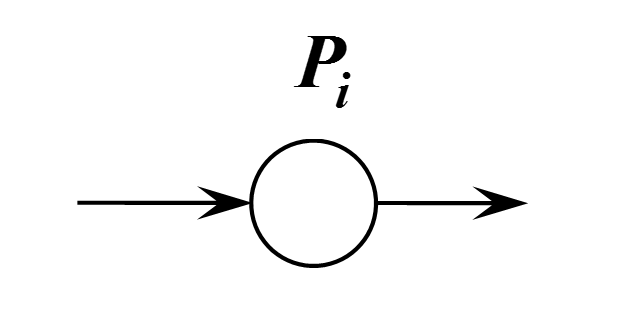
\includegraphics[width=0.3\textwidth]{place} \\ а)}
	\end{minipage}
	\hfill
	\begin{minipage}[ht]{0.49\linewidth}
		\center{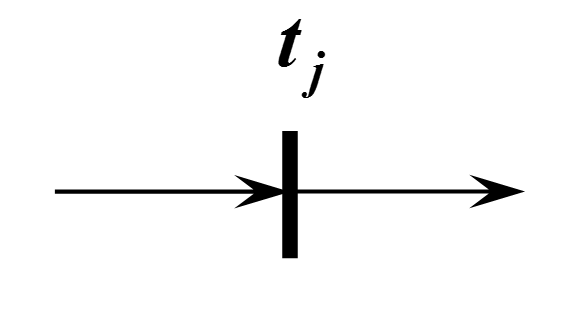
\includegraphics[width=0.3\linewidth]{tansition} \\ б)}
	\end{minipage}
	\caption{a) "--- Изображение позиции, б) "--- Изображение перехода. }
	\label{img:example}  
\end{figure}

Ориентированные дуги могут соединять только позиции и переходы в прямом и обратном направлении (свойство двудольности~\cite{piterson}). Сеть Петри является мультиграфом, так как допускается кратность дуг между позициями и переходами (вершинами графа). Пример сети Петри приведен на рисунке \ref{img:petri-net}.

\begin{figure}[h!]
	\center{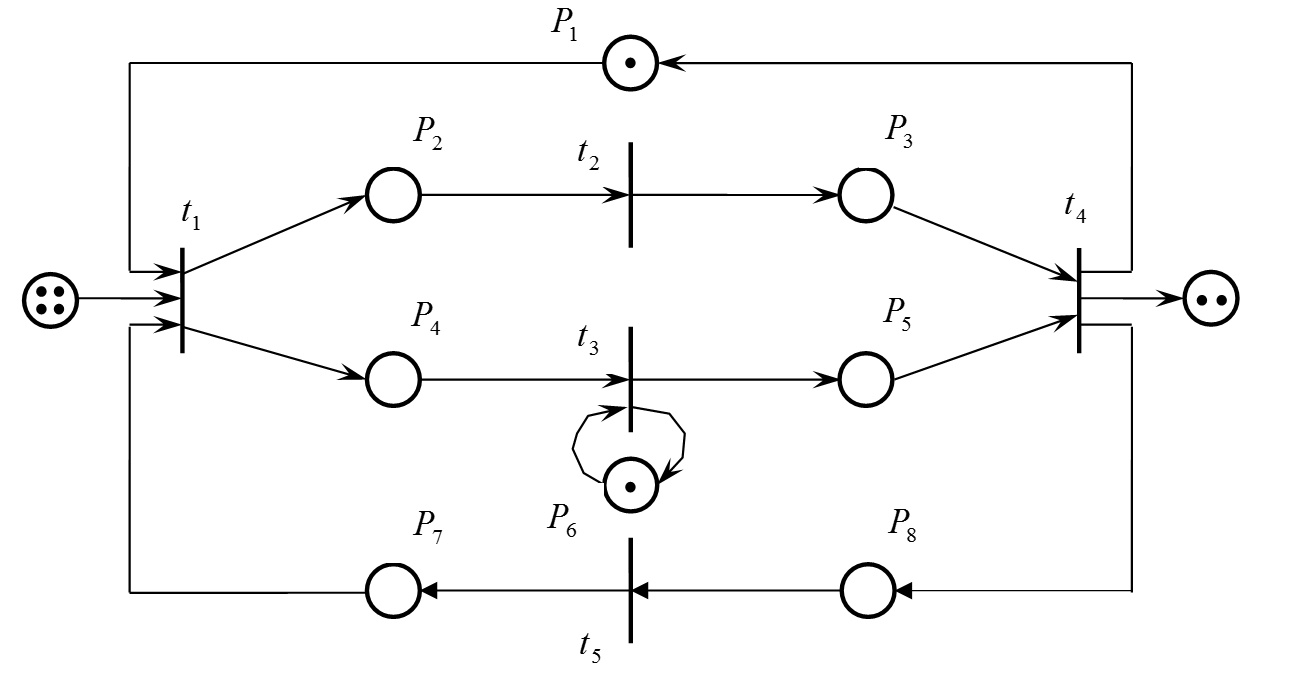
\includegraphics[width=0.7\textwidth]{petri-net}}
	\caption{Пример сети петри.}
	\label{img:petri-net}
\end{figure}

Сетью Петри принято называть тройку $<G, m_0, \rho>$  , где  $G\equiv<P, T, I, O>$ "--- граф сети Петри, $P$   "--- конечное множество позиций (или мест) сети, $T$ "--- конечное множество переходов сети, $P \cap T = \varnothing$. $I, O:T\rightarrow P^{()}$  "--- функции, задающие комплекты входных и, соответственно, выходных позиций переходов сети (здесь $P^{()}$  "--- множество всевозможных конечных комплектов элементов мно-жества $P$ ). $M \cong P^{()}$ "--- множество всевозможных состояний сети (маркировок).  $m_0 \in M$ "--- начальная маркировка сети, задающая начальное состояние сети, $\rho:T\rightarrow C$ "--- функция раскраски, возможно частичная, где $C$  "--- множество красок.

Сеть называется ограниченной, если $ (\forall p \in P) (\exists k \in \textit{nat}) (\forall m \in \mu_0) (m(p) \leq k)$, то есть множество достижимых в сети маркировок конечно.

Ограниченная сеть Петри $S$ на множестве позиций $P$, $|P|\in \mathbb{N}_0$, может быть представлена следуюзим образом~\cite{falkTheory}:\\ 
$ S \subseteq P^{()} \times (P^{()} \times P^{()}) $.

Неограниченная сеть Петри $S$ на  $P$, $|P|\in \mathbb{N}_0$:	$ S \subseteq P^{()} \times 2^{P^{()} \times P^{()}} $.

Для любой сети Петри $S\equiv < m_0, T >,\;  m_0 \in P^{()}$ называется начальной разметкой сети, а направленное квазиотношение $T$ -- множество переходов сети.

Сети Петри рассматриваются с точностью до изоморфизма: две сети $S'\equiv<{m'}_0, T'>$ на $P'$ и $S''\equiv<{m''}_0, T''>$ на $P''$ изоморфны ($ S' \sim S'' $), если существует взаимооднозначное соответствие $ \varepsilon:P'\leftrightarrow P'' $, такое, что $ \varepsilon(T') = T'' $. Графическое представление сетей Петри хорошо известно и не нуждается в уточнении.

Бинарное отношение $\mathrm{T}(T)$ изменения разметок на множестве $P^{()}$ разметок сети Петри $S\equiv < m_0, T >$:
\begin{center}
	$\mathrm{T}(T)\cong\{<p',p''-p_1+p_2>|<p_1,p_2> \in T \wedge p_1\leq p''\}.$
\end{center}

История поведения стандартной ограниченной сети Петри $S\equiv < m_0, T >$: кортеж $<m_0,m_1,...,m_k>$, 
такой, что $(\forall i \in 1..k)(<m_{i-1}, m_i> \in \mathrm{T}(T))$.

Множество всех возможных историй поведения сети Петри $S$ обозначим $\mu(S)$.

Две сети Петри $S_1$ и $S_2$ эквивалентны, если $\mu(S_1) \sim \mu(S_2)$ (т.е. существует взаимно-однозначное соответствие $\varepsilon:P'\leftrightarrow P''$, такое, что $\varepsilon(\mu(S')) = \mu(S'')$).


В качестве графического средства сети Петри могут использоваться для наглядного представления моделируемой системы. 
Вводимое в этих сетях понятие фишек позволяет моделировать динамику функционирования систем и параллельные процессы. 
В качестве математического средства аналитическое представление сети Петри позволяет составлять уравнения состояния, алгебраические уравнения и другие математические соотношения, описывающие динамику систем~\cite{radioElect}.

\section{Сети Петри со строгой дисциплиной изменения разметок}
Бинарное отношение $\bar{\mathrm{T}}(T)$ строгого изменения разметок на множестве $P^{()}$ 
разметок сети в сети Петри $S\equiv < m_0, T >$~\cite{falkTheory}:
\begin{equation}
\begin{multlined}
\bar{\mathrm{T}}(T)\cong\{<p',p''-p_1+p_2>|<p_1,p_2> \in T \wedge p_1\leq p'' \wedge\\
\wedge (\exists<{p'}_1, {p''}_2> \in T)(p_1 < {p'}_1 \wedge {p'}_1 \leq p'') \}.
\end{multlined}
\end{equation}

История поведения ограниченной сети Петри $S\equiv < m_0, T >$ со строгим изменением разметок: кортеж  $<m_0, m_1, ..., m_k>$, 
такой, что\\ $(\forall i \in 1..k)(<m_{i-1}, m_i> \in \bar{\mathrm{T}}(T))$.

Пусть задана стандартная ограниченная сеть Петри $S\equiv < m_0, T >$. Пополним множество $P$ ее позиций множеством $P_G$ новых элементов,
взаимно-однозначно соответствующих переходам из $G$: $P'\cong P\cup P_G$,\\ 
$P_G\cong \{p_t|(t\in T)\wedge (p_t \notin P)\}$. Искомую ограниченную сеть Петри со строгой дисциплиной изменения разметок 
обозначим $S'\equiv  < {m'}_0, T >$:\\
${m'}_0\cong m_0 +\displaystyle\sum_{p_t\in P_G}c_{p_t}$,
$T'\cong\{\alpha'+c_{p_{<\alpha', \alpha''>}}, \alpha'' +c_{<p_{\alpha', \alpha''>}}|<\alpha', \alpha''> \in T\} $.
Доказательство эквивалентности сетей $S$ и $S'$ очевидно.
\section{Динамические вычислительные сети}
% Для отображения символа в большом варианте использовать \displaystyle
Пусть 
$ D = \displaystyle\bigcup_{\theta\in\Theta} D_\theta $  - многосортный \textit{универсум данных},  
где $\Theta$ - конечное множество \textit{сортов} данных, 
$D_\theta$ - подмножество \textit{данных} сорта $\theta\in\Theta$.\\
Будем считать, что одним из таких сортов данных является сорт \textit{nat}, такой, что $D_{\textit{nat}} \cong \mathbb{N}_0$.
Функциональным базисом будем называть конечное множество  $ B $   всюду определенных вычислимых~\cite{falkTheory} функций вида:\\
$ \beta: \displaystyle\bigtimes_{i'\in 1..m'}D_{\theta'_{i'}} \rightarrow \displaystyle\bigtimes_{i''\in 1..m''}D_{\theta''_{i''}} $, $ m', m'' \in \mathbb{N}_0 $  , 
где  $ <m', m''> $   называется арностью функции $ \beta $  , а  $ <\nu', \nu''> $ -- ее типом, где $ \nu'\in \Theta^{<m'>}, \nu''\in \Theta^{m''} $
.

\textit{ Динамической вычислительной сетью} (\textbf{ДВС}) в функциональном базисе $B$ 
назовем пару $<\bar{\Sigma}, \dot{S}>$, где $\overline{\Sigma}$ 
- конечное множество классов сетей ДВС, $\dot{S}$ - аксиома ДВС.

Каждый класс $\Sigma$ характеризуется: 
уникальным именем  $\dot{\Sigma}$, 
типом функции 
$< |\bar{\theta}'(\dot{\Sigma})|, |\bar{\theta}''(\dot{\Sigma})|>$
,  и конечным упорядоченным множеством $S^*(\dot{\Sigma})$
\textit{образов сетей} этого класса.
Тип или арность может указываться,
при необходимости, в виде правого верхнего индекса.

Все образцы сетей из $S^*(\dot{\Sigma})$ имеют тот же тип, а, следовательно,
и арность, что и сам класс $\Sigma$.
Тип или арность образца сети   $S\in\bar{S}(\dot{\Sigma})$ ,
при необходимости, также может указываться в виде его правого верхнего индекса.

Образец сети  $S\in{S^*(\dot{\Sigma})}$   в общем случае имеет вид:
\begin{center}
	$S\cong<P, \delta, I, O, T_T, T_H, \nu', \nu'', I_T, O_T, \sigma, \rho, \varphi_T, \lambda_I, \lambda_O, \mu_0> $,где
\end{center}
\begin{itemize}
	\item $P$ 
	"--- конечное множество элементов\footnote{Используемый здесь термин «элемент сети» является, во многом, аналогом терминов «позиция» или «место» в теории сетей Петри и «точка сети» в теории направленных отношений.}
	образца сети,
	
	\item $\delta:P \rightarrow \Theta$  "--- задает сорта элементов образца сети,
	\item  $I, O \in P^{<>}$ "--- кортежи входных и выходных элементов образца сети, \mbox{$<\delta(I), \delta(O)>$}  "---  тип, а $<|I|, |O|>$   "--- арность образца сети,
	
	\item $T_T$ 
	"--- конечное множество терминальных переходов,
	
	\item $T_H$ 
	"--- конечное множество нетерминальных переходов,
	$T_T \cap T_H = \varnothing$  , $T\cong  T_T \cup T_H$ , $T \cap P = \varnothing$ ,
	
	\item	для всех $ t \in T$  : $I_T(t) \in P^{<\nu'(t)>}$ ,
	$ O_T(t) \in P^{\nu''(t)} $  ;\\
	$<\nu'(t), \nu''(t)>$   "--- \textit{арность перехода}  $ t \in T $   ( $ \nu', \nu'':T\rightarrow\mathbb{N}_0 $ ),\\
	$ <\delta(I_T(t)), \delta(O_T(t))> $  "--- \textit{тип перехода} $t$  , 
	
	\item $ \sigma:T_H \rightarrow \{ \dot{\Sigma}\;| \;\Sigma \in \bar{\Sigma} \} $ (сопоставляет имена классов сетей-объектов нетерминальным переходам),
	
	\item $ \rho:T_H \rightarrow \mathbb{Q}_0 $ (задает \textit{временные сдвиги} для нетерминальных переходов),
	
	\item $ \omega:T_H \rightarrow P $(задает \textit{управляющие входы} нетерминальных переходов), для всех  $ t \in T_H $  $ \delta(\omega(t)) = \textit{nat} $   ;
	
	\item $ \varphi_T:T_T \rightarrow B $ – \textit{семантика} терминальных переходов, причем для всех  $ t \in T_T $    тип  $\varphi_T(t)$    равен  $ <\delta(I_T(t)), \delta(O_T(t))> $  ,
	
	\item $ \lambda_I:\{ <t, i'>|\; t\in T_T \wedge i' \in 1..\nu'(t) \} \rightarrow \mathbb{Q}_0 $ и
	
	\item $ \lambda_O:\{ <t, i''>|\; t\in T_T \wedge i'' \in 1..\nu''(t) \} \rightarrow \mathbb{Q}_0 $ задают «задержки» входных и выходных связей терминальных переходов с элементами образца сети,
	
	\item $ \mu_0 \in M_S $ , 
	где $ M_S \cong \{ \mu\;| \; (\forall p \in P)(\mu(p) \in (D_{\delta(p)} \times \mathbb{Q}_0)^{()} \} $.
	Компонент $ \mu_0 $    является, в определенном смысле, аналогом понятия маркировки сетей Петри,
	в связи с чем множество  $ M_S $   будем тоже называть \textit{множеством возможных маркировок} сети,
	а $\mu_0$   – ее \textit{начальной маркировкой}.
	Не ограничивая общности, далее будем считать, что для любой маркировки  $\mu\in M_S$
	все комплекты  $\mu(p)$  (для всех $p \in P$ ) представлены кортежами вида 
	$ < <d_1, \tau_1>, ..., <d_{|\mu(p)|}, \tau_{|\mu(p)|} > $  , 
	построенными из элементов соответствующего комплекта так, 
	что компоненты кортежей упорядочены по неубыванию вторых компонентов пар 
	(т.е. $ (\forall i\in 1..|\mu|-1) (\tau_i \leq \tau_{i+1}) $~). 
\end{itemize}

\newtheorem{com}{Замечание}
\begin{com}\label{izomorph}
	Заметим, что образцы сетей рассматриваются с точностью до $(P, T_T, T_H)$-изоморфизма.
\end{com}

\textit{ Аксиома} или, по-иному, инициальное состояние $\dot{S}$ ДВС (корень дерева состояний) -- один из образцов некоторого класса $\Sigma \in \bar{\Sigma}$.


\section{Процессы реального времени}
Абстрактный процесс в системе определяется как последовательность $ \langle P_0, P_1, ...\rangle $   состояний системы, а процесс реального времени – как последовательность упорядоченных пар $ \langle P_i, t_i \rangle, i\in N_0 $\footnote{$ \mathbb{N}_0 \cong \{0, 1, 2, \dots\}$}, представленных состояниями системы и временами переходов системы в эти состояния, причем времена в последовательности строго упорядочены по возрастанию. 
Далее мы будем рассматривать только процессы реального времени. 
В общем случае для недетерминированных систем процессы представлены конечными или бесконечными путями из корня дерева процессов.
Корень дерева процессов представляет собой пару $ \langle P(t_0), 0 \rangle $ , где $ P_0 $  – начальное состояние всех заданных этим деревом процессов в момент времени  $ t_0 = 0 $. 

\subsection{Шкала времени} \label{sec:time}
В понятии процесса используется понятие времени, как абстрактного, представленного номерами в образующей процесс последовательности, так и реального, представленного элементами числовой шкалы времени, которая представлена линейно упорядоченным множеством моментов времени и, желательно: 
\begin{itemize}
	\item включает минимальное и максимальное значения, 
	\item имеет разрешимые предикаты сравнения ($ <, \leq, =, \geq, > $),
	\item является плотной, в которой для любых различных моментов времени $ t^{'} $  и $ t^{''} $  , таких, что $ t^{'}<t^{''} $ , существует момент времени $ t $ , такой, что  $ t^{'}<t $  и $ t<t^{''} $ .
\end{itemize}

Не ограничивая общности, будем в качестве удовлетворяющей этим требованиям шкалы времени рассматривать множество $ \breve{\mathbb{Q}} = \mathbb{Q} \cup \{\omega\} $, где $ \mathbb{Q}=\mathbb{Q}_+\cup \{0\} $, $ \mathbb{Q}_+ $~- множество положительных рациональных чисел, $ 0 $ - минимальное значение:$ (\forall t \in \mathbb{Q}_+) (0<t) $ , $ \omega $ - несобственное значение, время, неограниченно отдаленное в будущем: $ (\forall t \in \mathbb{Q}) (t<\omega) $. 
Сохраняя основные свойства арифметических операций, доопределим естественным образом для элементов множества $ \breve{\mathbb{Q}} $ указанные отношения $ <, \leq, =, \geq, > $ и арифметические операции сложения, вычитания, умножения и деления, за исключением некоторых случаев: $ \omega/\omega $ , $ 0/0 $ , $ 0*\omega $  и вычитания из меньшего значения большего. 
Заметим, что положительные рациональные числа представляются упорядоченными парами положительных натуральных чисел, в общем случае неоднозначно. Каноническое представление предполагает, что эти числа являются взаимно-простыми. Через $ \tau $   будем далее обозначать текущее время в системе, через $ t\in \mathbb{Q} $  --- произвольный момент времени.

\section{Понятие эпизода}
В основе предлагаемых далее определений мы используем понятие эпизода. 
Эпизоды задаются их типами и двумя моментами времени: начала и завершения (более точно определено ниже). 
Неформально, эпизоды~--- некие сущности (объекты, свойства и т.п.) на интервалах рассматриваемой шкалы времени. 
Интервал~--- упорядоченная пара $ \langle t^{'}, t^{''}\rangle $ моментов времени, такая, что  $ t^{'}<t^{''} $. 
Состояние системы в любой момент времени $ t $ определяется как неупорядоченный набор (комплект, конечное мультимножество) не завершившихся к этому времени эпизодов.

Пусть $ \phi \equiv \langle e, \theta \rangle $~--- эпизод. 
Первый компонент представляет тип эпизода из не более чем счетного множества  $ E $  типов эпизодов в рассматриваемой системе. 
Важную роль в описании частных случаев определения процессов в системах играет структуризация множества типов эпизодов. 
Разбиение типа на два компонента практически не ограничивает общности: $ E \equiv E_B \times E_D $. 
Первый компонент типа определяет возможные события в системе, приводящие к изменению ее состояния, а второй~--- наполняет их конкретным содержанием. 
Для всех  $ \langle e_B, e_D \rangle \in E $  полагаем, что $ e_B $~--- структурный атрибут эпизода, $ e_D $~--- его информационный атрибут. 
Практически полезной является и дальнейшая детализация структурного атрибута: полагаем, что $ e_B \equiv \langle e_B^{'}, e_B^{''} \rangle $ , где $ e_B^{'} $~--- один из группирующих эпизоды контейнеров, к которому <<относится>> (или, иначе говоря, в котором <<находится>> эпизод), а $ e_B^{''} $~--- сорт (или тег) эпизода, уточняющий средства оперирования с информационными атрибутами (аналог понятия типа или класса информационных объектов в языках программирования). 
В частном случае, сорт эпизода может однозначно определяться его контейнером. 
В свою очередь, сорт эпизода определяет множество возможных значений его информационного атрибута. 
Предполагается, что множество значений информационного атрибута любого сорта содержит неопределенное значение  $ \perp $.

Второй компонент эпизода $ \theta \equiv \langle t^{'} t^{''} \rangle \in \mathbb{Q} \times \breve{\mathbb{Q}} $, $ t^{'}<t^{''} $ задает временные характеристики конкретного эпизода: $ t^{'}\in \mathbb{Q} $  определяет начало эпизода на шкале времени; $ t^{''}\in \breve{\mathbb{Q}} $ , если эпизод завершен ($ \tau \geq t^{''} $), то это --- конец эпизода, иначе эпизод полагается незавершенным, и $ \delta \cong t^{''}-t^{'} > 0 $ понимается как предельно возможная длительность незавершенного эпизода (если $ t^{''}=\omega $ , то возможная длительность эпизода сверху не ограничена). 

\section{Состояние вычислительной системы}

Пусть $ D = \bigcup_{\theta \in \Theta} D_\theta $ - многосортный универсум данных, где $ \Theta $ - конечное множество сортов данных, $ D_\theta $ - подмножество данных сорты $ \theta \in \Theta $.

\textit{Структура вычислительной сети} $ S = \langle C, I \rangle $ представляет собой пару множеств. 

Первое из них, $ C $ --- множество контейнеров эпизодов. 
Контейнер $ c \in C $ определяется множеством сортов эпизодов, допустимых для помещения в контейнер.

Второе множество, $ I $ - интерфейс системы. 
Интерфейс состоит из элементов интерфейса и определяет возможные изменения в системе. 
Элемент $ i  = \langle \beta, R \rangle $ представляет собой пару из функции функционального базиса $ \beta \in B $ (определим его далее) и множества требований к атрибутам эпизодов, необходимых для срабатывания элемента интерфейса.
Для всех $ \langle r_B, r_T \rangle \in R $ полагаем, что $ r_B $ - требование к структурному атрибуту эпизода (к контейнеру и (или) сорту), а $ r_T \in \mathbb{Q}_+ $ - требуемое минимальное время жизни эпизода по отношению к текущему моменту времени $ \tau $.

\textit{Состоянием вычислительной сети} в момент времени $ t \in \mathbb{Q} $ называется $ P_t = \langle E_t, S_t \rangle $, где
\begin{itemize}
	\item $ E_t $ --- множество незавершенных эпизодов в момент времени $ t $;
	\item $ S_t $ --- структура вычислительной системы в момент времени $ t $.
\end{itemize}


\section{Интерфейс системы}
Согласно нашему первоначальному замыслу, основные объекты в определении понятия системы~--- состояние системы, интерфейс, элемент интерфейса – должны были быть определены как неупорядоченные наборы, соответственно, незавершенных эпизодов, элементов интерфейса и требований к структурным атрибутам эпизодов, необходимых для срабатывания элементов интерфейса, составляющих события в системе, приводящие к изменению ее состояния. 
Однако, вследствие этого появляется значительная неопределенность в поведении системы, выражающаяся в чрезмерном разрастании дерева процессов. Для предотвращения этого мы отказались от концепции неупорядоченности, что позволило ввести в описание систем разного рода приоритеты, устраняющие во многом недетерминированность поведения систем. 
Фактически, неоднозначность появляется только вследствие маловероятного случайного совпадения времени готовности к срабатывания структурно не связанных элементов интерфейса и по причине сознательного отказа от учета информационных атрибутов эпизодов в формировании событий в системе, оставив только их влияние на результат~--- возможные изменения состояния системы.

В дальнейшем будем различать два варианта систем: с последовательным и параллельным интерфейсом.

В общем случае интерфейс рассматривается как упорядоченное множество элементов интерфейса, причём требование упорядоченности используется, во-первых, для приоритетного применения элементов интерфейса для систем с последовательным интерфейсом, во-вторых, для приоритетного распределения эпизодов состояния системы при одновременном срабатывании комплекта элементов интерфейса для систем с параллельным интерфейсом.

\subsubsection{Дисциплины выбора эпизодов}
Каждый отдельный элемент интерфейса определяет кортеж требований к элементам соответствующего ему набора эпизодов, а именно, к их контейнерам и (или) сортам, а также к временам их появления (к началам эпизодов) по отношению к минимально возможному моменту предполагаемого их совместного срабатывания – в виде так называемой <<выдержки>> эпизодов с областью значений $ \mathbb{Q}_+ $ . 
Если из эпизодов текущего состояния системы можно сформировать соответствующий элементу интерфейса кортеж эпизодов, то будем говорить, что элемент интерфейса готов к срабатыванию в рассматриваемый момент времени. 
Ограничить разнообразие удовлетворяющих этим требованиям комплектов эпизодов можно дополнительно заданием для конкретного элемента интерфейса одной из дисциплин выбора эпизодов из текущего состояния системы: 
\begin{itemize}
	\item \textit{FIFO} (First In First Out) --- предпочтение отдается <<старым>> эпизодам (с более ранним началом);
	\item \textit{LIFO} (Last In First Out) --- предпочтение отдается <<молодым>> эпизодам (с более поздним началом);
	\item \textit{FEFO} (First End First Out) --- предпочтение отдаётся эпизодам с более ранним временем окончания.
\end{itemize} 

\subsection{Задание интерфейса}

В простейшем случае элементы действующего в текущий момент времени интерфейса могут быть заданы путем их непосредственного перечисления, разумеется, если их конечное число.
В более общем случае, который в этой работе не рассматривается, интерфейс задается в форме некоторой схемы – выражений формального языка, содержащих, возможно, свободные вхождения переменных с известными областями значений, причем возможными значениями этих выражений являются отдельные элементы интерфейса, а само множество значений является рекурсивно-перечислимым (и, в общем случае, может быть бесконечным). 

\subsection{Последовательные и параллельные интерфейсы}

Для систем с последовательным интерфейсом отдельные его элементы анализируются на возможность срабатывания в порядке их перечисления, вплоть до первого готового к срабатыванию в ближайший момент времени по отношению к времени предыдущего события. 
Очевидно, что \textit{в один и тот же момент времени может произойти последовательное срабатывание нескольких элементов интерфейса} в порядке их перечисления.

Для систем с параллельным интерфейсом отдельные элементы интерфейса определяют только возможность событий в системе. 
В системе выделяются готовые к одновременному срабатыванию в некоторый момент времени подкомплекты эпизодов текущего состояния системы при условии ненаступления до этого других событий. 
Поэтому переход к новому состоянию системы, как и для систем с последовательным интерфейсом, может стать реальным только для возможных событий с минимальным ожидаемым временем. 
Если это время окажется больше максимально возможного времени окончания хотя бы одного из выбранных эпизодов, то для определения готовности всё следует повторить для состояния, в котором удалены такие эпизоды. 
Если требуемых комплектов эпизодов нет, то процесс завершается; в противном случае рассматривается готовность к одновременному срабатыванию всевозможных комплектов указанных комплектов эпизодов для отдельных элементов параллельного интерфейса. 
Хотя при этом рассматривается возможность выделения в состоянии системы комплектов эпизодов на основе <<смешивания>> упорядоченных по времени выдержки подкортежей требований к различным значениям структурных атрибутов эпизодов, необходимых для срабатывания элементов интерфейса, однако, сам выбор конкретных эпизодов и сама возможность такого выбора с полученным на первом этапе минимально возможным временем срабатывания могут оказаться иными даже при условии сохранения дисциплины выбора, индивидуально заданной для каждого элемента интерфейса. 
Полагаем, что фактически смогут реализоваться только \textbf{максимальные} из этих готовых к совместному срабатыванию комплектов элементов интерфейса. 
Реализуемый таким образом \textit{принцип максимально возможного параллелизма} в поведении системы позволяет исключить из рассмотрения события с одним и тем же временем. 
Если таких максимальных суммарных комплектов более одного, то поведение системы становится недетерминированным, и, как было сказано ранее, оно формализуется в виде дерева процессов: происходит его ветвление, вершина текущего состояния системы будет иметь несколько потомков, по одному для каждого указанного выше случая. 
Каждый из вариантов определяет и свой результат соответствующего события, т.е. изменения состояния системы и действующего интерфейса.

\section{События}
Изменение состояний системы в автоматной модели определяется как ее текущим состоянием, так и действующим интерфейсом, который устанавливает взаимосвязь эпизодов и, в общем случае, сам тоже может изменяться при переходах системы к новым состояниям. В каждый момент времени действующий интерфейс определяет для текущего состояния системы возможность событий, в результате которых могут измениться и состояние системы, и действующий интерфейс. 
Событие~--- переход системы в новое состояние, который характеризуется моментом времени этого перехода и определяется временем ближайшего предшествующего события, текущим состоянием системы и действующим интерфейсом эпизодов. 
Первопричинами основных событий являются: 
\begin{enumerate}[label=\arabic*)]
	\item появление в состоянии системы наборов (комплектов) эпизодов, необходимые требования к которым и определяет действующий интерфейс;
	\item в динамических системах~--- подключение к системе определенным образом модифицированных копий подсистем. 
\end{enumerate}
Изменение состояния системы возможно также в связи с достижением максимально возможного времени окончания некоторого эпизода, в этом случае такой эпизод исключается из состояния системы и не может влиять на последующие события. 
Информационный атрибут такого завершенного эпизода полагается равным $ \perp $. 

\section{Результат события}
Перейдем к краткому рассмотрению результата события – к изменениям состояния системы.

Пусть процесс не обрывается и $ t_{i+1} $  – время очередного события. 
Во-первых, из состояния $ P_i $ уже исключены эпизоды, время максимально возможного окончания которых меньше $ t_{i+1} $. 
Участвующие в событии эпизоды также исключаются из состояния системы. 
Каждый из участвовавших в событии элемент интерфейса порождает, с учетом его кратности вхождения в реализованный в событии комплект элементов интерфейса, комплект новых эпизодов, добавляемых к текущему состоянию системы (после указанных выше удалений эпизодов). 
Для каждого нового эпизода задаются полностью (и контейнеры, и сорта) структурные атрибуты, <<задержка>> (число из $ \mathbb{Q} $ ), результат сложения которого с  $ t_{i+1} $  дает начало этого эпизода, и еще одно число из $ \breve{\mathbb{Q}} $ . 
Если оно равно нулю, то длительность нового эпизода не ограничена сверху (параметр <<конец эпизода>> получает значение $ \omega $ ), в противном случае он задает положительную длительность эпизода, а значение параметра <<конец эпизода>> получается сложением длительности с началом эпизода. 
Все это, в сочетании с требованием задания положительных значений для выдержек, гарантирует отсутствие готовности к срабатыванию в момент времени $ t_{i+1} $ новых, появившихся в результате рассматриваемого события, эпизодов в состоянии системы. 

\subsection{Функциональный базис системы}
В общем случае все характеристики новых эпизодов определяются как значения заданных для каждого элемента интерфейса функций из функционального базиса системы, согласованных по сортам аргументов с сортами входных эпизодов элемента интерфейса. 
Значениями аргументов этих функций выступают значения информационных атрибутов выделенных в состоянии системы $ P_i $ участвующих в событии эпизодов для рассматриваемого элемента интерфейса. 
Именно с целью установления соответствия аргументов и их значений перечисление требований к эпизодам уже в элементе интерфейса осуществляется в некотором порядке, т.е. в форме кортежа. 

В частном случае, структурные атрибуты (контейнеры, сорта) и максимально возможные времена окончаний новых эпизодов задаются непосредственно в элементе интерфейса, если всем сортам эпизодов сопоставлены одноэлементные множества возможных значений информационных атрибутов. 

Существует несколько альтернатив определения функции в функциональном базисе, которые зависят от параметров системы.
\begin{itemize}
	\item Функции вида $ \beta : \bigtimes_{i \in 1..n} D_{\theta_i} \rightarrow \bigtimes_{i \in 1..m} D_{\theta_i}$, где $ \langle
	n,m \rangle $ - арность функции, а $ \langle \nu, \mu \rangle $ - тип функции, где $ \nu \in \Theta^{<n>}, \mu \in \Theta^{<m>} $. 
	Такие функции лишь выполняют вычисления с использованием информационных атрибутов. 
	Результат функции --- кортеж новых информационных атрибутов фиксированной длины. 
	Для создания новых эпизодов элемент интерфейса должен также содержать кортеж связей элемента с контейнерами результатов $ <c, t_l, t_d >, c \in C, t_l \in \mathbb{\mathbb{Q}}_+, t_d \in \mathbb{\mathbb{Q}} $, где $ c $ - контейнер результата, $ t_l $ - время задержки эпизода, $ t_d $ - длительность эпизода.
	\item Функции вида $ \beta : \bigtimes_{i \in 1..n} D_{\theta_i} \rightarrow \bigtimes_{i \in 1..m} (D_{\theta_i} \times \mathbb{Q}_+ \times \mathbb{Q})$. 
	В отличае от предыдущего вида, время задержки эпизода и длительность эпизода здесь определяется функцией.
	Элемент интерфейса же содержит исключительно информацию о целевых контейнерах для результатов функции.
	\item Функции вида $ \beta : (\bigtimes_{i \in 1..n} D_{\theta_i}) \times \mathbb{Q}_+ \rightarrow \bigtimes_{i \in 1..m} \Phi_{\theta_i}$, где $ \Phi $ - множество возможных эпизодов.
	В качестве последнего входного параметра используется $ \tau $ - текущее время в система.
	Заранее неизвестно, в какой контейнер попадёт новый эпизод, однако сохраняются арность и тип функции.
	\item Функции вида $ \beta : (\bigtimes_{i \in 1..n} D_{\theta_i}) \times \mathbb{Q}_+ \rightarrow \Phi^{\langle\rangle}$.
	Для таких функций возможно не только определять значение структурного атрибута результатов, но и управлять своей арностью.
\end{itemize}

\subsection{Изменение структуры}
Описанные события не приводят к изменению структуры системы, множество используемых контейнеров ограничено множеством контейнеров, фигурирующих в начальном состоянии системы и ее интерфейсе. 
Такие системы будем называть статическими. 
Для описания поведения динамических систем, интерфейс которых может изменяться во времени, а множества используемых контейнеров неограниченно расширяться, нужны совсем иные пути формализации для реализации этих возможностей. 
Не претендуя на общность, мы предлагаем дополнительно ввести в качестве элементов интерфейсов динамических систем так называемые нетерминальные элементы, в то время как рассмотренные ранее будем называть терминальными элементами интерфейсов. 

Если для терминальных элементов интерфейса эффект выражается в создании новых эпизодов и сохранении действующего интерфейса, то в результате срабатывания нетерминального элемента интерфейса происходят структурные изменения: могут появиться новые элементы интерфейса, могут появиться не только новые эпизоды в состоянии системы, но и новые контейнеры. 
Вопрос же об удалении из рассмотрения некоторых контейнеров и элементов интерфейса должен решаться подобно тому, как решается проблема <<сборки мусора>> для памяти типа <<куча>>.

Динамическая система представлена в виде конечного множества именованных подсистем, каждая из которых задана тройкой~--- начальным состоянием, начальным интерфейсом и упорядоченным конечным подмножеством контейнеров подсистемы, элементы которого будем называть контактами подсистемы. 
Контейнеры подсистемы, не вошедшие в число контактов, при срабатывании нетерминального элемента интерфейса и подключении к системе этой подсистемы будут представлять новые контейнеры, отличные от всех ранее используемых в системе. 
Механизм порождения новых контейнеров аналогичен процессу выделения новых ячеек в памяти типа <<куча>> и, в какой-то мере, операции замены связанной переменной в формальных системах с операторами, связывающих вхождения операторной переменной в терм, к которому применяется оператор (например в $ \lambda $-исчислении). 
Вершина дерева процессов (начальное состояние системы) представлена начальным состоянием выделенной базовой подсистемы (аксиомы). 
Предполагается возможность в дальнейшем подключений к системе любых подсистем, в том числе и подсистемы-аксиомы. 
Множество имен всех подсистем образуют особый сорт $ \Delta $ значений информационных атрибутов эпизодов.

В текущем интерфейсе всякий нетерминальный элемент представлен следующей информацией: 
\begin{enumerate}[label=\arabic*)]
	\item контейнером, наличие в котором эпизода сорта $ \Delta $   может привести к срабатыванию этого нетерминального элемента, 
	\item  выдержкой, играющей ту же роль, что и выдержки эпизодов в терминальных элементах интерфейса, 
	\item  кортежем контейнеров текущего состояния системы, элементы которого будем называть контактами рассматриваемого нетерминального элемента текущего интерфейса (заметим, что один и тот же контейнер может входить неоднократно в указанный кортеж), 
	\item  функцией, аргументом которой является имя подсистемы, а значением – задержка подключения соответствующей подсистемы из множества $ \mathbb{Q} $ .
\end{enumerate}  

Условием возможного срабатывания нетерминального элемента интерфейса в момент времени $ t_{i+1} = t_i + \delta $, где $ \delta $~--- указанная для этого элемента <<выдержка>>, является просто наличие в состоянии системы соответствующего эпизода сорта $ \Delta $ в указанном контейнере. 
В результате срабатывания нетерминального элемента интерфейса происходит подключение к системе некоторой подсистемы, имя которой определяется информационным атрибутом эпизодов, что приводит к изменениям основных компонентов состояния системы, помимо тех, которые вносятся в результате возможного одновременного срабатывания терминальных элементов интерфейса. 
Одна из основных проблем определения процедуры подключения подсистемы состоит в том, чтобы она исключала возможность в момент времени подключения срабатывания новых элементов обновленного интерфейса. 
Кроме того, при одновременном срабатывании нескольких нетерминальных элементов результат подключения нескольких подсистем не должен зависеть от порядка их реализации.

\subsection{Подключение подсистемы}
Опишем вначале способ подключения к системе некоторой одной подсистемы.

Как было сказано ранее, для выполнения подключений каждая подсистема, помимо ее начального состояния и начального интерфейса, содержит контактную информацию для ее подключений, и, в свою очередь, всякий нетерминальный элемент действующего интерфейса системы также содержит свою контактную информацию. 
Контактная информация позволяет установить связь между контейнерами основной системы и контейнерами подключаемой подсистемы путем замены контейнеров в подключаемой системе на соответствующие (согласно порядкам перечисления контактов) контейнеры основной системы; 
именно для того, чтобы при подключении не возникла возможность <<ложных>>, не реализованных к моменту подключения срабатываний элементов действующего интерфейса системы, соответствующая контактная информация в основной системе задается в форме кортежа используемых в ней контейнеров, а в подключаемой подсистеме --- в форме упорядоченного подмножества используемых в ней контейнеров, причем для остальных контейнеров подключаемой подсистемы производится их замена на новые контейнеры, не используемые ранее в основной системе. 
При подключении подсистемы начала всех эпизодов во всех ее контейнерах формируются путем сложений их начал и, соответственно, концов, заданных в начальном состоянии подключаемой подсистемы, времени события, включающего срабатывание рассматриваемого нетерминального элемента основной системы, и задержки подключения соответствующей подсистемы при срабатывании конкретного нетерминального элемента интерфейса системы. 
Так как новый интерфейс системы в результате срабатывания нетерминального элемента пополняется элементами интерфейса подключаемой подсистемы, то указанное изменение временных параметров подключаемых к состоянию системы эпизодов подсистемы не может привести к готовности в тот же момент времени к срабатыванию как <<старых>>, так и <<новых>> элементов интерфейса. 
Очевидно, что, так как интерфейс подключаемых подсистем может тоже содержать нетерминальные элементы, то в системе может неограниченно увеличиваться количество используемых контейнеров и элементов интерфейса, а описанная далее <<сборка мусора>> в системе может приводить к удалению <<лишних>> эпизодов, контейнеров и элементов интерфейса.

В общем случае, событие, приводящее к изменению состояния системы в момент времени $ t_{i+1} $ , может включать одновременное срабатывание не только нескольких терминальных элементов интерфейса, но и нескольких его нетерминальных элементов. 
Подключение одной подсистемы предполагает следующую последовательность шагов:
\begin{itemize}
	\item создание рабочих копий начального состояния и начального интерфейса выбранной для подключения подсистемы (далее под состоянием и интерфейсом подключаемой подсистемы будем понимать эти копии); 
	изменение в состоянии и интерфейсе подключаемой подсистемы временных параметров эпизодов так, как было описано выше;
	\item замена различных контейнеров в состоянии и интерфейсе подключаемой подсистемы на различные новые контейнеры, не используемые ни в текущем состоянии и интерфейсе системы, ни в начальном состоянии и интерфейсе подключаемой подсистемы;
	\item замена всех контейнеров в состоянии и интерфейсе подключаемой подсистемы, входящих в число ее контактов, на соответствующие им по порядку контейнеры в кортеже контактов рассматриваемого нетерминального элемента интерфейса (если в последнем <<хватает>> контактов);
	\item к состоянию системы присоединяется состояние подключаемой подсистемы (путем сложения представляющих их комплектов), а к интерфейсу систем добавляется интерфейс подключаемой подсистемы (путем конкатенации представляющих их кортежей).
\end{itemize}

\section{Вывод}
Описанная модель является развитием теории Динамических вычислительных сетей, основанной на сетях Петри. 
Однако, в данном формализме предполагается наличие принципиальных отличий даже базовых понятий теории сетей Петри: 
\begin{itemize}
	\item отказ от переходов с пустым комплектом входных позиций: в этом отношении мы обобщаем принцип <<отсутствие необходимых ресурсов (фишек) не может служить основанием каких-либо событий (переходов).>> Это требование, не являясь принципиальным при рассмотрении поведения системы в абстрактном времени, для реального времени является принципиальным;
	\item введение линейных порядков на множествах входных и выходных позиций переходов уже используются во многих обобщениях формализма сетей Петри, и, как следствие, замена понятий <<комплект входных (выходных) позиций перехода>> на понятия <<кортеж входных (выходных) эпизодов для элемента интерфейса>>. В  нашем формализме это необходимо для описания роли информационных атрибутов эпизодов;
	\item срабатывание переходов (элементов интерфейса) управляется не только наличием фишек во входных позициях (контейнерах), а и их окраской (сортами эпизодов);
	\item изменение состояний происходят в реальном, а не в абстрактом (модельном) времени, что позволяет строить более адекватные модели поведения реальных систем;
	\item в нашем подходе всегда реализуется максимально возможный параллелизм срабатывания элементов интерфейса (в базовой модели сетей Петри не допускается одновременное срабатывание нескольких переходов, а моделирование этого делает сеть неоправданно громоздкой). Этот подход позволяет в системе реального времени избавиться от возможности нескольких событий с одинаковым временем;
	\item наконец, главное: сами рассматриваемые нами системы являются динамическими, могут структурно меняться во времени и иметь при функционировании априори не ограниченную сложность.
Изменением терминологии хочется подчеркнуть следующую основную цель публикации: описание проходящих в реальном времени параллельных вычислительных процессов в динамических системах с априори не ограниченной сложностью \cite{Falk}.
\end{itemize}



%\chapter{Теоретическое введение}
	\label{chap:one}
\section{Сети Петри}

Формально сеть Петри определена в~\cite{piterson} и представляет собой двудольный граф с двумя родами вершин: одни вершины называются позициями, другие
называются переходами. 
Построение моделей систем в виде сетей Петри заключается в следующем.
\begin{enumerate}
	\item 	Моделируемые процессы описываются множеством событий (действий) и условий определяющих возможность наступления этих событий, а также причинно-следственными отношениями, устанавливаемыми на множестве пар "события-условия".
	\item Определяются события-действия, последовательность выполнения которых управляется состояниями системы. Состояния системы задаются множеством условий, формируемых в виде предикатов. Количественно условия характеризуются величиной, которая выражается числами натурального ряда.
\item Условия, в зависимости от значений их количественных характеристик, могут выполняться или нет. Выполнение условий обеспечивает возможность реализации событий. Условия, с фактом выполнения которых связывается возможность реализации событий, называются предусловиями. Реализация события обеспечивает возможность выполнения других условий, находящихся с предусловиями в причинно-следственной связи. Эти условия называются постусловиями.
\end{enumerate}

В сетях Петри условия - это позиции, а события - переходы. В соответствии с этим граф сети Петри является двудольным ориентированным мультиграфом. Изображение позиции и перехода на графе показано на рисунке \ref{img:example}.

\begin{figure}[h!]
	\begin{minipage}[ht]{0.49\linewidth}
		\center{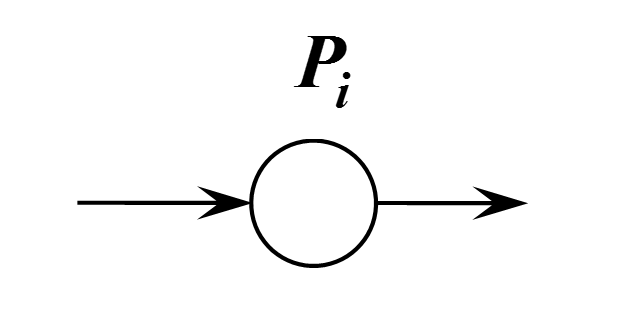
\includegraphics[width=0.3\textwidth]{place} \\ а)}
	\end{minipage}
	\hfill
	\begin{minipage}[ht]{0.49\linewidth}
		\center{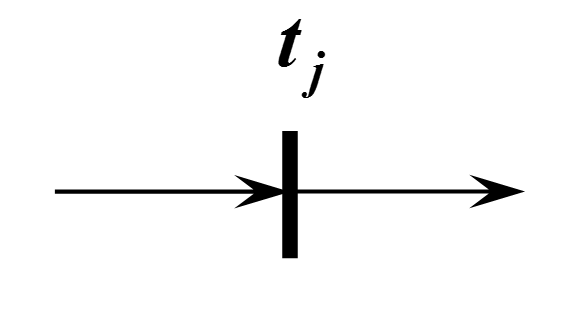
\includegraphics[width=0.3\linewidth]{tansition} \\ б)}
	\end{minipage}
	\caption{a) "--- Изображение позиции, б) "--- Изображение перехода. }
	\label{img:example}  
\end{figure}

Ориентированные дуги могут соединять только позиции и переходы в прямом и обратном направлении (свойство двудольности~\cite{piterson}). Сеть Петри является мультиграфом, так как допускается кратность дуг между позициями и переходами (вершинами графа). Пример сети Петри приведен на рисунке \ref{img:petri-net}.

\begin{figure}[h!]
	\center{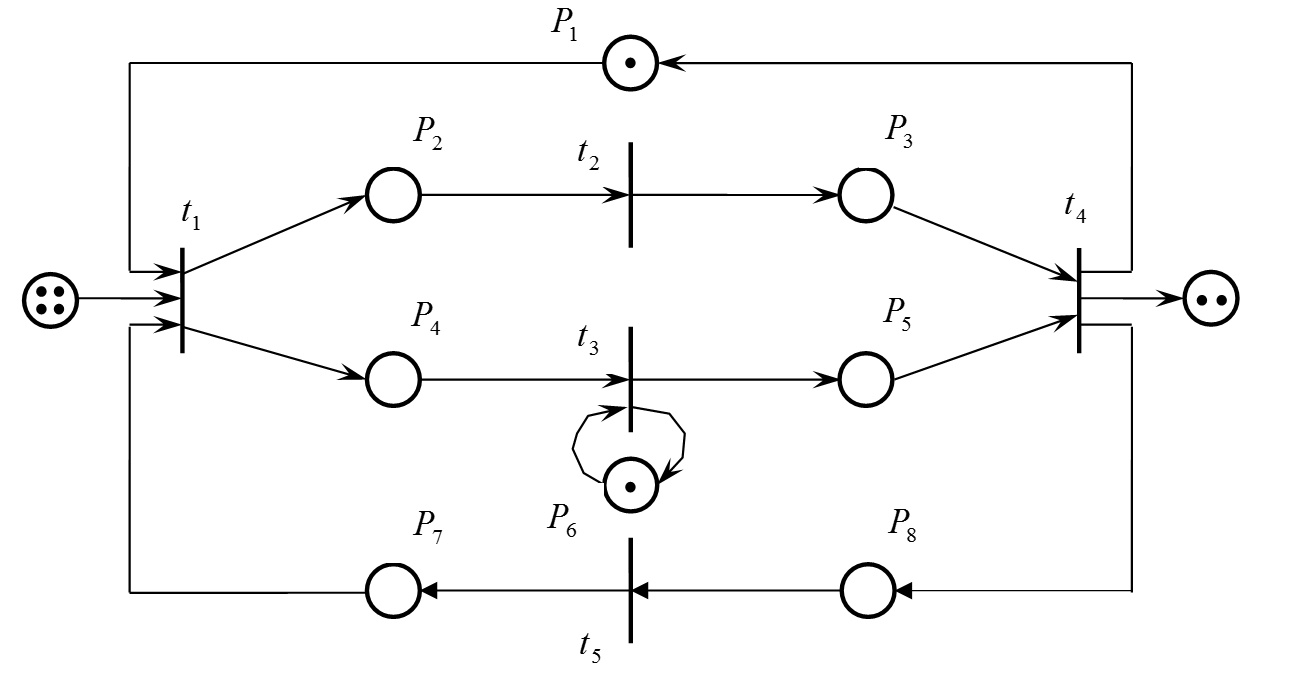
\includegraphics[width=0.7\textwidth]{petri-net}}
	\caption{Пример сети петри.}
	\label{img:petri-net}
\end{figure}

Сетью Петри принято называть тройку $<G, m_0, \rho>$  , где  $G\equiv<P, T, I, O>$ "--- граф сети Петри, $P$   "--- конечное множество позиций (или мест) сети, $T$ "--- конечное множество переходов сети, $P \cap T = \varnothing$. $I, O:T\rightarrow P^{()}$  "--- функции, задающие комплекты входных и, соответственно, выходных позиций переходов сети (здесь $P^{()}$  "--- множество всевозможных конечных комплектов элементов мно-жества $P$ ). $M \cong P^{()}$ "--- множество всевозможных состояний сети (маркировок).  $m_0 \in M$ "--- начальная маркировка сети, задающая начальное состояние сети, $\rho:T\rightarrow C$ "--- функция раскраски, возможно частичная, где $C$  "--- множество красок.

Сеть называется ограниченной, если $ (\forall p \in P) (\exists k \in \textit{nat}) (\forall m \in \mu_0) (m(p) \leq k)$, то есть множество достижимых в сети маркировок конечно.

Ограниченная сеть Петри $S$ на множестве позиций $P$, $|P|\in \mathbb{N}_0$, может быть представлена следуюзим образом~\cite{falkTheory}:\\ 
$ S \subseteq P^{()} \times (P^{()} \times P^{()}) $.

Неограниченная сеть Петри $S$ на  $P$, $|P|\in \mathbb{N}_0$:	$ S \subseteq P^{()} \times 2^{P^{()} \times P^{()}} $.

Для любой сети Петри $S\equiv < m_0, T >,\;  m_0 \in P^{()}$ называется начальной разметкой сети, а направленное квазиотношение $T$ -- множество переходов сети.

Сети Петри рассматриваются с точностью до изоморфизма: две сети $S'\equiv<{m'}_0, T'>$ на $P'$ и $S''\equiv<{m''}_0, T''>$ на $P''$ изоморфны ($ S' \sim S'' $), если существует взаимооднозначное соответствие $ \varepsilon:P'\leftrightarrow P'' $, такое, что $ \varepsilon(T') = T'' $. Графическое представление сетей Петри хорошо известно и не нуждается в уточнении.

Бинарное отношение $\mathrm{T}(T)$ изменения разметок на множестве $P^{()}$ разметок сети Петри $S\equiv < m_0, T >$:
\begin{center}
	$\mathrm{T}(T)\cong\{<p',p''-p_1+p_2>|<p_1,p_2> \in T \wedge p_1\leq p''\}.$
\end{center}

История поведения стандартной ограниченной сети Петри $S\equiv < m_0, T >$: кортеж $<m_0,m_1,...,m_k>$, 
такой, что $(\forall i \in 1..k)(<m_{i-1}, m_i> \in \mathrm{T}(T))$.

Множество всех возможных историй поведения сети Петри $S$ обозначим $\mu(S)$.

Две сети Петри $S_1$ и $S_2$ эквивалентны, если $\mu(S_1) \sim \mu(S_2)$ (т.е. существует взаимно-однозначное соответствие $\varepsilon:P'\leftrightarrow P''$, такое, что $\varepsilon(\mu(S')) = \mu(S'')$).


В качестве графического средства сети Петри могут использоваться для наглядного представления моделируемой системы. 
Вводимое в этих сетях понятие фишек позволяет моделировать динамику функционирования систем и параллельные процессы. 
В качестве математического средства аналитическое представление сети Петри позволяет составлять уравнения состояния, алгебраические уравнения и другие математические соотношения, описывающие динамику систем~\cite{radioElect}.

\section{Сети Петри со строгой дисциплиной изменения разметок}
Бинарное отношение $\bar{\mathrm{T}}(T)$ строгого изменения разметок на множестве $P^{()}$ 
разметок сети в сети Петри $S\equiv < m_0, T >$~\cite{falkTheory}:
\begin{equation}
\begin{multlined}
\bar{\mathrm{T}}(T)\cong\{<p',p''-p_1+p_2>|<p_1,p_2> \in T \wedge p_1\leq p'' \wedge\\
\wedge (\exists<{p'}_1, {p''}_2> \in T)(p_1 < {p'}_1 \wedge {p'}_1 \leq p'') \}.
\end{multlined}
\end{equation}

История поведения ограниченной сети Петри $S\equiv < m_0, T >$ со строгим изменением разметок: кортеж  $<m_0, m_1, ..., m_k>$, 
такой, что\\ $(\forall i \in 1..k)(<m_{i-1}, m_i> \in \bar{\mathrm{T}}(T))$.

Пусть задана стандартная ограниченная сеть Петри $S\equiv < m_0, T >$. Пополним множество $P$ ее позиций множеством $P_G$ новых элементов,
взаимно-однозначно соответствующих переходам из $G$: $P'\cong P\cup P_G$,\\ 
$P_G\cong \{p_t|(t\in T)\wedge (p_t \notin P)\}$. Искомую ограниченную сеть Петри со строгой дисциплиной изменения разметок 
обозначим $S'\equiv  < {m'}_0, T >$:\\
${m'}_0\cong m_0 +\displaystyle\sum_{p_t\in P_G}c_{p_t}$,
$T'\cong\{\alpha'+c_{p_{<\alpha', \alpha''>}}, \alpha'' +c_{<p_{\alpha', \alpha''>}}|<\alpha', \alpha''> \in T\} $.
Доказательство эквивалентности сетей $S$ и $S'$ очевидно.
\section{Динамические вычислительные сети}
% Для отображения символа в большом варианте использовать \displaystyle
Пусть 
$ D = \displaystyle\bigcup_{\theta\in\Theta} D_\theta $  - многосортный \textit{универсум данных},  
где $\Theta$ - конечное множество \textit{сортов} данных, 
$D_\theta$ - подмножество \textit{данных} сорта $\theta\in\Theta$.\\
Будем считать, что одним из таких сортов данных является сорт \textit{nat}, такой, что $D_{\textit{nat}} \cong \mathbb{N}_0$.
Функциональным базисом будем называть конечное множество  $ B $   всюду определенных вычислимых~\cite{falkTheory} функций вида:\\
$ \beta: \displaystyle\bigtimes_{i'\in 1..m'}D_{\theta'_{i'}} \rightarrow \displaystyle\bigtimes_{i''\in 1..m''}D_{\theta''_{i''}} $, $ m', m'' \in \mathbb{N}_0 $  , 
где  $ <m', m''> $   называется арностью функции $ \beta $  , а  $ <\nu', \nu''> $ -- ее типом, где $ \nu'\in \Theta^{<m'>}, \nu''\in \Theta^{m''} $
.

\textit{ Динамической вычислительной сетью} (\textbf{ДВС}) в функциональном базисе $B$ 
назовем пару $<\bar{\Sigma}, \dot{S}>$, где $\overline{\Sigma}$ 
- конечное множество классов сетей ДВС, $\dot{S}$ - аксиома ДВС.

Каждый класс $\Sigma$ характеризуется: 
уникальным именем  $\dot{\Sigma}$, 
типом функции 
$< |\bar{\theta}'(\dot{\Sigma})|, |\bar{\theta}''(\dot{\Sigma})|>$
,  и конечным упорядоченным множеством $S^*(\dot{\Sigma})$
\textit{образов сетей} этого класса.
Тип или арность может указываться,
при необходимости, в виде правого верхнего индекса.

Все образцы сетей из $S^*(\dot{\Sigma})$ имеют тот же тип, а, следовательно,
и арность, что и сам класс $\Sigma$.
Тип или арность образца сети   $S\in\bar{S}(\dot{\Sigma})$ ,
при необходимости, также может указываться в виде его правого верхнего индекса.

Образец сети  $S\in{S^*(\dot{\Sigma})}$   в общем случае имеет вид:
\begin{center}
	$S\cong<P, \delta, I, O, T_T, T_H, \nu', \nu'', I_T, O_T, \sigma, \rho, \varphi_T, \lambda_I, \lambda_O, \mu_0> $,где
\end{center}
\begin{itemize}
	\item $P$ 
	"--- конечное множество элементов\footnote{Используемый здесь термин «элемент сети» является, во многом, аналогом терминов «позиция» или «место» в теории сетей Петри и «точка сети» в теории направленных отношений.}
	образца сети,
	
	\item $\delta:P \rightarrow \Theta$  "--- задает сорта элементов образца сети,
	\item  $I, O \in P^{<>}$ "--- кортежи входных и выходных элементов образца сети, \mbox{$<\delta(I), \delta(O)>$}  "---  тип, а $<|I|, |O|>$   "--- арность образца сети,
	
	\item $T_T$ 
	"--- конечное множество терминальных переходов,
	
	\item $T_H$ 
	"--- конечное множество нетерминальных переходов,
	$T_T \cap T_H = \varnothing$  , $T\cong  T_T \cup T_H$ , $T \cap P = \varnothing$ ,
	
	\item	для всех $ t \in T$  : $I_T(t) \in P^{<\nu'(t)>}$ ,
	$ O_T(t) \in P^{\nu''(t)} $  ;\\
	$<\nu'(t), \nu''(t)>$   "--- \textit{арность перехода}  $ t \in T $   ( $ \nu', \nu'':T\rightarrow\mathbb{N}_0 $ ),\\
	$ <\delta(I_T(t)), \delta(O_T(t))> $  "--- \textit{тип перехода} $t$  , 
	
	\item $ \sigma:T_H \rightarrow \{ \dot{\Sigma}\;| \;\Sigma \in \bar{\Sigma} \} $ (сопоставляет имена классов сетей-объектов нетерминальным переходам),
	
	\item $ \rho:T_H \rightarrow \mathbb{Q}_0 $ (задает \textit{временные сдвиги} для нетерминальных переходов),
	
	\item $ \omega:T_H \rightarrow P $(задает \textit{управляющие входы} нетерминальных переходов), для всех  $ t \in T_H $  $ \delta(\omega(t)) = \textit{nat} $   ;
	
	\item $ \varphi_T:T_T \rightarrow B $ – \textit{семантика} терминальных переходов, причем для всех  $ t \in T_T $    тип  $\varphi_T(t)$    равен  $ <\delta(I_T(t)), \delta(O_T(t))> $  ,
	
	\item $ \lambda_I:\{ <t, i'>|\; t\in T_T \wedge i' \in 1..\nu'(t) \} \rightarrow \mathbb{Q}_0 $ и
	
	\item $ \lambda_O:\{ <t, i''>|\; t\in T_T \wedge i'' \in 1..\nu''(t) \} \rightarrow \mathbb{Q}_0 $ задают «задержки» входных и выходных связей терминальных переходов с элементами образца сети,
	
	\item $ \mu_0 \in M_S $ , 
	где $ M_S \cong \{ \mu\;| \; (\forall p \in P)(\mu(p) \in (D_{\delta(p)} \times \mathbb{Q}_0)^{()} \} $.
	Компонент $ \mu_0 $    является, в определенном смысле, аналогом понятия маркировки сетей Петри,
	в связи с чем множество  $ M_S $   будем тоже называть \textit{множеством возможных маркировок} сети,
	а $\mu_0$   – ее \textit{начальной маркировкой}.
	Не ограничивая общности, далее будем считать, что для любой маркировки  $\mu\in M_S$
	все комплекты  $\mu(p)$  (для всех $p \in P$ ) представлены кортежами вида 
	$ < <d_1, \tau_1>, ..., <d_{|\mu(p)|}, \tau_{|\mu(p)|} > $  , 
	построенными из элементов соответствующего комплекта так, 
	что компоненты кортежей упорядочены по неубыванию вторых компонентов пар 
	(т.е. $ (\forall i\in 1..|\mu|-1) (\tau_i \leq \tau_{i+1}) $~). 
\end{itemize}

\newtheorem{com}{Замечание}
\begin{com}\label{izomorph}
	Заметим, что образцы сетей рассматриваются с точностью до $(P, T_T, T_H)$-изоморфизма.
\end{com}

\textit{ Аксиома} или, по-иному, инициальное состояние $\dot{S}$ ДВС (корень дерева состояний) -- один из образцов некоторого класса $\Sigma \in \bar{\Sigma}$.


\section{Процессы реального времени}
Абстрактный процесс в системе определяется как последовательность $ \langle P_0, P_1, ...\rangle $   состояний системы, а процесс реального времени – как последовательность упорядоченных пар $ \langle P_i, t_i \rangle, i\in N_0 $\footnote{$ \mathbb{N}_0 \cong \{0, 1, 2, \dots\}$}, представленных состояниями системы и временами переходов системы в эти состояния, причем времена в последовательности строго упорядочены по возрастанию. 
Далее мы будем рассматривать только процессы реального времени. 
В общем случае для недетерминированных систем процессы представлены конечными или бесконечными путями из корня дерева процессов.
Корень дерева процессов представляет собой пару $ \langle P(t_0), 0 \rangle $ , где $ P_0 $  – начальное состояние всех заданных этим деревом процессов в момент времени  $ t_0 = 0 $. 

\subsection{Шкала времени} \label{sec:time}
В понятии процесса используется понятие времени, как абстрактного, представленного номерами в образующей процесс последовательности, так и реального, представленного элементами числовой шкалы времени, которая представлена линейно упорядоченным множеством моментов времени и, желательно: 
\begin{itemize}
	\item включает минимальное и максимальное значения, 
	\item имеет разрешимые предикаты сравнения ($ <, \leq, =, \geq, > $),
	\item является плотной, в которой для любых различных моментов времени $ t^{'} $  и $ t^{''} $  , таких, что $ t^{'}<t^{''} $ , существует момент времени $ t $ , такой, что  $ t^{'}<t $  и $ t<t^{''} $ .
\end{itemize}

Не ограничивая общности, будем в качестве удовлетворяющей этим требованиям шкалы времени рассматривать множество $ \breve{\mathbb{Q}} = \mathbb{Q} \cup \{\omega\} $, где $ \mathbb{Q}=\mathbb{Q}_+\cup \{0\} $, $ \mathbb{Q}_+ $~- множество положительных рациональных чисел, $ 0 $ - минимальное значение:$ (\forall t \in \mathbb{Q}_+) (0<t) $ , $ \omega $ - несобственное значение, время, неограниченно отдаленное в будущем: $ (\forall t \in \mathbb{Q}) (t<\omega) $. 
Сохраняя основные свойства арифметических операций, доопределим естественным образом для элементов множества $ \breve{\mathbb{Q}} $ указанные отношения $ <, \leq, =, \geq, > $ и арифметические операции сложения, вычитания, умножения и деления, за исключением некоторых случаев: $ \omega/\omega $ , $ 0/0 $ , $ 0*\omega $  и вычитания из меньшего значения большего. 
Заметим, что положительные рациональные числа представляются упорядоченными парами положительных натуральных чисел, в общем случае неоднозначно. Каноническое представление предполагает, что эти числа являются взаимно-простыми. Через $ \tau $   будем далее обозначать текущее время в системе, через $ t\in \mathbb{Q} $  --- произвольный момент времени.

\section{Понятие эпизода}
В основе предлагаемых далее определений мы используем понятие эпизода. 
Эпизоды задаются их типами и двумя моментами времени: начала и завершения (более точно определено ниже). 
Неформально, эпизоды~--- некие сущности (объекты, свойства и т.п.) на интервалах рассматриваемой шкалы времени. 
Интервал~--- упорядоченная пара $ \langle t^{'}, t^{''}\rangle $ моментов времени, такая, что  $ t^{'}<t^{''} $. 
Состояние системы в любой момент времени $ t $ определяется как неупорядоченный набор (комплект, конечное мультимножество) не завершившихся к этому времени эпизодов.

Пусть $ \phi \equiv \langle e, \theta \rangle $~--- эпизод. 
Первый компонент представляет тип эпизода из не более чем счетного множества  $ E $  типов эпизодов в рассматриваемой системе. 
Важную роль в описании частных случаев определения процессов в системах играет структуризация множества типов эпизодов. 
Разбиение типа на два компонента практически не ограничивает общности: $ E \equiv E_B \times E_D $. 
Первый компонент типа определяет возможные события в системе, приводящие к изменению ее состояния, а второй~--- наполняет их конкретным содержанием. 
Для всех  $ \langle e_B, e_D \rangle \in E $  полагаем, что $ e_B $~--- структурный атрибут эпизода, $ e_D $~--- его информационный атрибут. 
Практически полезной является и дальнейшая детализация структурного атрибута: полагаем, что $ e_B \equiv \langle e_B^{'}, e_B^{''} \rangle $ , где $ e_B^{'} $~--- один из группирующих эпизоды контейнеров, к которому <<относится>> (или, иначе говоря, в котором <<находится>> эпизод), а $ e_B^{''} $~--- сорт (или тег) эпизода, уточняющий средства оперирования с информационными атрибутами (аналог понятия типа или класса информационных объектов в языках программирования). 
В частном случае, сорт эпизода может однозначно определяться его контейнером. 
В свою очередь, сорт эпизода определяет множество возможных значений его информационного атрибута. 
Предполагается, что множество значений информационного атрибута любого сорта содержит неопределенное значение  $ \perp $.

Второй компонент эпизода $ \theta \equiv \langle t^{'} t^{''} \rangle \in \mathbb{Q} \times \breve{\mathbb{Q}} $, $ t^{'}<t^{''} $ задает временные характеристики конкретного эпизода: $ t^{'}\in \mathbb{Q} $  определяет начало эпизода на шкале времени; $ t^{''}\in \breve{\mathbb{Q}} $ , если эпизод завершен ($ \tau \geq t^{''} $), то это --- конец эпизода, иначе эпизод полагается незавершенным, и $ \delta \cong t^{''}-t^{'} > 0 $ понимается как предельно возможная длительность незавершенного эпизода (если $ t^{''}=\omega $ , то возможная длительность эпизода сверху не ограничена). 

\section{Состояние вычислительной системы}

Пусть $ D = \bigcup_{\theta \in \Theta} D_\theta $ - многосортный универсум данных, где $ \Theta $ - конечное множество сортов данных, $ D_\theta $ - подмножество данных сорты $ \theta \in \Theta $.

\textit{Структура вычислительной сети} $ S = \langle C, I \rangle $ представляет собой пару множеств. 

Первое из них, $ C $ --- множество контейнеров эпизодов. 
Контейнер $ c \in C $ определяется множеством сортов эпизодов, допустимых для помещения в контейнер.

Второе множество, $ I $ - интерфейс системы. 
Интерфейс состоит из элементов интерфейса и определяет возможные изменения в системе. 
Элемент $ i  = \langle \beta, R \rangle $ представляет собой пару из функции функционального базиса $ \beta \in B $ (определим его далее) и множества требований к атрибутам эпизодов, необходимых для срабатывания элемента интерфейса.
Для всех $ \langle r_B, r_T \rangle \in R $ полагаем, что $ r_B $ - требование к структурному атрибуту эпизода (к контейнеру и (или) сорту), а $ r_T \in \mathbb{Q}_+ $ - требуемое минимальное время жизни эпизода по отношению к текущему моменту времени $ \tau $.

\textit{Состоянием вычислительной сети} в момент времени $ t \in \mathbb{Q} $ называется $ P_t = \langle E_t, S_t \rangle $, где
\begin{itemize}
	\item $ E_t $ --- множество незавершенных эпизодов в момент времени $ t $;
	\item $ S_t $ --- структура вычислительной системы в момент времени $ t $.
\end{itemize}


\section{Интерфейс системы}
Согласно нашему первоначальному замыслу, основные объекты в определении понятия системы~--- состояние системы, интерфейс, элемент интерфейса – должны были быть определены как неупорядоченные наборы, соответственно, незавершенных эпизодов, элементов интерфейса и требований к структурным атрибутам эпизодов, необходимых для срабатывания элементов интерфейса, составляющих события в системе, приводящие к изменению ее состояния. 
Однако, вследствие этого появляется значительная неопределенность в поведении системы, выражающаяся в чрезмерном разрастании дерева процессов. Для предотвращения этого мы отказались от концепции неупорядоченности, что позволило ввести в описание систем разного рода приоритеты, устраняющие во многом недетерминированность поведения систем. 
Фактически, неоднозначность появляется только вследствие маловероятного случайного совпадения времени готовности к срабатывания структурно не связанных элементов интерфейса и по причине сознательного отказа от учета информационных атрибутов эпизодов в формировании событий в системе, оставив только их влияние на результат~--- возможные изменения состояния системы.

В дальнейшем будем различать два варианта систем: с последовательным и параллельным интерфейсом.

В общем случае интерфейс рассматривается как упорядоченное множество элементов интерфейса, причём требование упорядоченности используется, во-первых, для приоритетного применения элементов интерфейса для систем с последовательным интерфейсом, во-вторых, для приоритетного распределения эпизодов состояния системы при одновременном срабатывании комплекта элементов интерфейса для систем с параллельным интерфейсом.

\subsubsection{Дисциплины выбора эпизодов}
Каждый отдельный элемент интерфейса определяет кортеж требований к элементам соответствующего ему набора эпизодов, а именно, к их контейнерам и (или) сортам, а также к временам их появления (к началам эпизодов) по отношению к минимально возможному моменту предполагаемого их совместного срабатывания – в виде так называемой <<выдержки>> эпизодов с областью значений $ \mathbb{Q}_+ $ . 
Если из эпизодов текущего состояния системы можно сформировать соответствующий элементу интерфейса кортеж эпизодов, то будем говорить, что элемент интерфейса готов к срабатыванию в рассматриваемый момент времени. 
Ограничить разнообразие удовлетворяющих этим требованиям комплектов эпизодов можно дополнительно заданием для конкретного элемента интерфейса одной из дисциплин выбора эпизодов из текущего состояния системы: 
\begin{itemize}
	\item \textit{FIFO} (First In First Out) --- предпочтение отдается <<старым>> эпизодам (с более ранним началом);
	\item \textit{LIFO} (Last In First Out) --- предпочтение отдается <<молодым>> эпизодам (с более поздним началом);
	\item \textit{FEFO} (First End First Out) --- предпочтение отдаётся эпизодам с более ранним временем окончания.
\end{itemize} 

\subsection{Задание интерфейса}

В простейшем случае элементы действующего в текущий момент времени интерфейса могут быть заданы путем их непосредственного перечисления, разумеется, если их конечное число.
В более общем случае, который в этой работе не рассматривается, интерфейс задается в форме некоторой схемы – выражений формального языка, содержащих, возможно, свободные вхождения переменных с известными областями значений, причем возможными значениями этих выражений являются отдельные элементы интерфейса, а само множество значений является рекурсивно-перечислимым (и, в общем случае, может быть бесконечным). 

\subsection{Последовательные и параллельные интерфейсы}

Для систем с последовательным интерфейсом отдельные его элементы анализируются на возможность срабатывания в порядке их перечисления, вплоть до первого готового к срабатыванию в ближайший момент времени по отношению к времени предыдущего события. 
Очевидно, что \textit{в один и тот же момент времени может произойти последовательное срабатывание нескольких элементов интерфейса} в порядке их перечисления.

Для систем с параллельным интерфейсом отдельные элементы интерфейса определяют только возможность событий в системе. 
В системе выделяются готовые к одновременному срабатыванию в некоторый момент времени подкомплекты эпизодов текущего состояния системы при условии ненаступления до этого других событий. 
Поэтому переход к новому состоянию системы, как и для систем с последовательным интерфейсом, может стать реальным только для возможных событий с минимальным ожидаемым временем. 
Если это время окажется больше максимально возможного времени окончания хотя бы одного из выбранных эпизодов, то для определения готовности всё следует повторить для состояния, в котором удалены такие эпизоды. 
Если требуемых комплектов эпизодов нет, то процесс завершается; в противном случае рассматривается готовность к одновременному срабатыванию всевозможных комплектов указанных комплектов эпизодов для отдельных элементов параллельного интерфейса. 
Хотя при этом рассматривается возможность выделения в состоянии системы комплектов эпизодов на основе <<смешивания>> упорядоченных по времени выдержки подкортежей требований к различным значениям структурных атрибутов эпизодов, необходимых для срабатывания элементов интерфейса, однако, сам выбор конкретных эпизодов и сама возможность такого выбора с полученным на первом этапе минимально возможным временем срабатывания могут оказаться иными даже при условии сохранения дисциплины выбора, индивидуально заданной для каждого элемента интерфейса. 
Полагаем, что фактически смогут реализоваться только \textbf{максимальные} из этих готовых к совместному срабатыванию комплектов элементов интерфейса. 
Реализуемый таким образом \textit{принцип максимально возможного параллелизма} в поведении системы позволяет исключить из рассмотрения события с одним и тем же временем. 
Если таких максимальных суммарных комплектов более одного, то поведение системы становится недетерминированным, и, как было сказано ранее, оно формализуется в виде дерева процессов: происходит его ветвление, вершина текущего состояния системы будет иметь несколько потомков, по одному для каждого указанного выше случая. 
Каждый из вариантов определяет и свой результат соответствующего события, т.е. изменения состояния системы и действующего интерфейса.

\section{События}
Изменение состояний системы в автоматной модели определяется как ее текущим состоянием, так и действующим интерфейсом, который устанавливает взаимосвязь эпизодов и, в общем случае, сам тоже может изменяться при переходах системы к новым состояниям. В каждый момент времени действующий интерфейс определяет для текущего состояния системы возможность событий, в результате которых могут измениться и состояние системы, и действующий интерфейс. 
Событие~--- переход системы в новое состояние, который характеризуется моментом времени этого перехода и определяется временем ближайшего предшествующего события, текущим состоянием системы и действующим интерфейсом эпизодов. 
Первопричинами основных событий являются: 
\begin{enumerate}[label=\arabic*)]
	\item появление в состоянии системы наборов (комплектов) эпизодов, необходимые требования к которым и определяет действующий интерфейс;
	\item в динамических системах~--- подключение к системе определенным образом модифицированных копий подсистем. 
\end{enumerate}
Изменение состояния системы возможно также в связи с достижением максимально возможного времени окончания некоторого эпизода, в этом случае такой эпизод исключается из состояния системы и не может влиять на последующие события. 
Информационный атрибут такого завершенного эпизода полагается равным $ \perp $. 

\section{Результат события}
Перейдем к краткому рассмотрению результата события – к изменениям состояния системы.

Пусть процесс не обрывается и $ t_{i+1} $  – время очередного события. 
Во-первых, из состояния $ P_i $ уже исключены эпизоды, время максимально возможного окончания которых меньше $ t_{i+1} $. 
Участвующие в событии эпизоды также исключаются из состояния системы. 
Каждый из участвовавших в событии элемент интерфейса порождает, с учетом его кратности вхождения в реализованный в событии комплект элементов интерфейса, комплект новых эпизодов, добавляемых к текущему состоянию системы (после указанных выше удалений эпизодов). 
Для каждого нового эпизода задаются полностью (и контейнеры, и сорта) структурные атрибуты, <<задержка>> (число из $ \mathbb{Q} $ ), результат сложения которого с  $ t_{i+1} $  дает начало этого эпизода, и еще одно число из $ \breve{\mathbb{Q}} $ . 
Если оно равно нулю, то длительность нового эпизода не ограничена сверху (параметр <<конец эпизода>> получает значение $ \omega $ ), в противном случае он задает положительную длительность эпизода, а значение параметра <<конец эпизода>> получается сложением длительности с началом эпизода. 
Все это, в сочетании с требованием задания положительных значений для выдержек, гарантирует отсутствие готовности к срабатыванию в момент времени $ t_{i+1} $ новых, появившихся в результате рассматриваемого события, эпизодов в состоянии системы. 

\subsection{Функциональный базис системы}
В общем случае все характеристики новых эпизодов определяются как значения заданных для каждого элемента интерфейса функций из функционального базиса системы, согласованных по сортам аргументов с сортами входных эпизодов элемента интерфейса. 
Значениями аргументов этих функций выступают значения информационных атрибутов выделенных в состоянии системы $ P_i $ участвующих в событии эпизодов для рассматриваемого элемента интерфейса. 
Именно с целью установления соответствия аргументов и их значений перечисление требований к эпизодам уже в элементе интерфейса осуществляется в некотором порядке, т.е. в форме кортежа. 

В частном случае, структурные атрибуты (контейнеры, сорта) и максимально возможные времена окончаний новых эпизодов задаются непосредственно в элементе интерфейса, если всем сортам эпизодов сопоставлены одноэлементные множества возможных значений информационных атрибутов. 

Существует несколько альтернатив определения функции в функциональном базисе, которые зависят от параметров системы.
\begin{itemize}
	\item Функции вида $ \beta : \bigtimes_{i \in 1..n} D_{\theta_i} \rightarrow \bigtimes_{i \in 1..m} D_{\theta_i}$, где $ \langle
	n,m \rangle $ - арность функции, а $ \langle \nu, \mu \rangle $ - тип функции, где $ \nu \in \Theta^{<n>}, \mu \in \Theta^{<m>} $. 
	Такие функции лишь выполняют вычисления с использованием информационных атрибутов. 
	Результат функции --- кортеж новых информационных атрибутов фиксированной длины. 
	Для создания новых эпизодов элемент интерфейса должен также содержать кортеж связей элемента с контейнерами результатов $ <c, t_l, t_d >, c \in C, t_l \in \mathbb{\mathbb{Q}}_+, t_d \in \mathbb{\mathbb{Q}} $, где $ c $ - контейнер результата, $ t_l $ - время задержки эпизода, $ t_d $ - длительность эпизода.
	\item Функции вида $ \beta : \bigtimes_{i \in 1..n} D_{\theta_i} \rightarrow \bigtimes_{i \in 1..m} (D_{\theta_i} \times \mathbb{Q}_+ \times \mathbb{Q})$. 
	В отличае от предыдущего вида, время задержки эпизода и длительность эпизода здесь определяется функцией.
	Элемент интерфейса же содержит исключительно информацию о целевых контейнерах для результатов функции.
	\item Функции вида $ \beta : (\bigtimes_{i \in 1..n} D_{\theta_i}) \times \mathbb{Q}_+ \rightarrow \bigtimes_{i \in 1..m} \Phi_{\theta_i}$, где $ \Phi $ - множество возможных эпизодов.
	В качестве последнего входного параметра используется $ \tau $ - текущее время в система.
	Заранее неизвестно, в какой контейнер попадёт новый эпизод, однако сохраняются арность и тип функции.
	\item Функции вида $ \beta : (\bigtimes_{i \in 1..n} D_{\theta_i}) \times \mathbb{Q}_+ \rightarrow \Phi^{\langle\rangle}$.
	Для таких функций возможно не только определять значение структурного атрибута результатов, но и управлять своей арностью.
\end{itemize}

\subsection{Изменение структуры}
Описанные события не приводят к изменению структуры системы, множество используемых контейнеров ограничено множеством контейнеров, фигурирующих в начальном состоянии системы и ее интерфейсе. 
Такие системы будем называть статическими. 
Для описания поведения динамических систем, интерфейс которых может изменяться во времени, а множества используемых контейнеров неограниченно расширяться, нужны совсем иные пути формализации для реализации этих возможностей. 
Не претендуя на общность, мы предлагаем дополнительно ввести в качестве элементов интерфейсов динамических систем так называемые нетерминальные элементы, в то время как рассмотренные ранее будем называть терминальными элементами интерфейсов. 

Если для терминальных элементов интерфейса эффект выражается в создании новых эпизодов и сохранении действующего интерфейса, то в результате срабатывания нетерминального элемента интерфейса происходят структурные изменения: могут появиться новые элементы интерфейса, могут появиться не только новые эпизоды в состоянии системы, но и новые контейнеры. 
Вопрос же об удалении из рассмотрения некоторых контейнеров и элементов интерфейса должен решаться подобно тому, как решается проблема <<сборки мусора>> для памяти типа <<куча>>.

Динамическая система представлена в виде конечного множества именованных подсистем, каждая из которых задана тройкой~--- начальным состоянием, начальным интерфейсом и упорядоченным конечным подмножеством контейнеров подсистемы, элементы которого будем называть контактами подсистемы. 
Контейнеры подсистемы, не вошедшие в число контактов, при срабатывании нетерминального элемента интерфейса и подключении к системе этой подсистемы будут представлять новые контейнеры, отличные от всех ранее используемых в системе. 
Механизм порождения новых контейнеров аналогичен процессу выделения новых ячеек в памяти типа <<куча>> и, в какой-то мере, операции замены связанной переменной в формальных системах с операторами, связывающих вхождения операторной переменной в терм, к которому применяется оператор (например в $ \lambda $-исчислении). 
Вершина дерева процессов (начальное состояние системы) представлена начальным состоянием выделенной базовой подсистемы (аксиомы). 
Предполагается возможность в дальнейшем подключений к системе любых подсистем, в том числе и подсистемы-аксиомы. 
Множество имен всех подсистем образуют особый сорт $ \Delta $ значений информационных атрибутов эпизодов.

В текущем интерфейсе всякий нетерминальный элемент представлен следующей информацией: 
\begin{enumerate}[label=\arabic*)]
	\item контейнером, наличие в котором эпизода сорта $ \Delta $   может привести к срабатыванию этого нетерминального элемента, 
	\item  выдержкой, играющей ту же роль, что и выдержки эпизодов в терминальных элементах интерфейса, 
	\item  кортежем контейнеров текущего состояния системы, элементы которого будем называть контактами рассматриваемого нетерминального элемента текущего интерфейса (заметим, что один и тот же контейнер может входить неоднократно в указанный кортеж), 
	\item  функцией, аргументом которой является имя подсистемы, а значением – задержка подключения соответствующей подсистемы из множества $ \mathbb{Q} $ .
\end{enumerate}  

Условием возможного срабатывания нетерминального элемента интерфейса в момент времени $ t_{i+1} = t_i + \delta $, где $ \delta $~--- указанная для этого элемента <<выдержка>>, является просто наличие в состоянии системы соответствующего эпизода сорта $ \Delta $ в указанном контейнере. 
В результате срабатывания нетерминального элемента интерфейса происходит подключение к системе некоторой подсистемы, имя которой определяется информационным атрибутом эпизодов, что приводит к изменениям основных компонентов состояния системы, помимо тех, которые вносятся в результате возможного одновременного срабатывания терминальных элементов интерфейса. 
Одна из основных проблем определения процедуры подключения подсистемы состоит в том, чтобы она исключала возможность в момент времени подключения срабатывания новых элементов обновленного интерфейса. 
Кроме того, при одновременном срабатывании нескольких нетерминальных элементов результат подключения нескольких подсистем не должен зависеть от порядка их реализации.

\subsection{Подключение подсистемы}
Опишем вначале способ подключения к системе некоторой одной подсистемы.

Как было сказано ранее, для выполнения подключений каждая подсистема, помимо ее начального состояния и начального интерфейса, содержит контактную информацию для ее подключений, и, в свою очередь, всякий нетерминальный элемент действующего интерфейса системы также содержит свою контактную информацию. 
Контактная информация позволяет установить связь между контейнерами основной системы и контейнерами подключаемой подсистемы путем замены контейнеров в подключаемой системе на соответствующие (согласно порядкам перечисления контактов) контейнеры основной системы; 
именно для того, чтобы при подключении не возникла возможность <<ложных>>, не реализованных к моменту подключения срабатываний элементов действующего интерфейса системы, соответствующая контактная информация в основной системе задается в форме кортежа используемых в ней контейнеров, а в подключаемой подсистеме --- в форме упорядоченного подмножества используемых в ней контейнеров, причем для остальных контейнеров подключаемой подсистемы производится их замена на новые контейнеры, не используемые ранее в основной системе. 
При подключении подсистемы начала всех эпизодов во всех ее контейнерах формируются путем сложений их начал и, соответственно, концов, заданных в начальном состоянии подключаемой подсистемы, времени события, включающего срабатывание рассматриваемого нетерминального элемента основной системы, и задержки подключения соответствующей подсистемы при срабатывании конкретного нетерминального элемента интерфейса системы. 
Так как новый интерфейс системы в результате срабатывания нетерминального элемента пополняется элементами интерфейса подключаемой подсистемы, то указанное изменение временных параметров подключаемых к состоянию системы эпизодов подсистемы не может привести к готовности в тот же момент времени к срабатыванию как <<старых>>, так и <<новых>> элементов интерфейса. 
Очевидно, что, так как интерфейс подключаемых подсистем может тоже содержать нетерминальные элементы, то в системе может неограниченно увеличиваться количество используемых контейнеров и элементов интерфейса, а описанная далее <<сборка мусора>> в системе может приводить к удалению <<лишних>> эпизодов, контейнеров и элементов интерфейса.

В общем случае, событие, приводящее к изменению состояния системы в момент времени $ t_{i+1} $ , может включать одновременное срабатывание не только нескольких терминальных элементов интерфейса, но и нескольких его нетерминальных элементов. 
Подключение одной подсистемы предполагает следующую последовательность шагов:
\begin{itemize}
	\item создание рабочих копий начального состояния и начального интерфейса выбранной для подключения подсистемы (далее под состоянием и интерфейсом подключаемой подсистемы будем понимать эти копии); 
	изменение в состоянии и интерфейсе подключаемой подсистемы временных параметров эпизодов так, как было описано выше;
	\item замена различных контейнеров в состоянии и интерфейсе подключаемой подсистемы на различные новые контейнеры, не используемые ни в текущем состоянии и интерфейсе системы, ни в начальном состоянии и интерфейсе подключаемой подсистемы;
	\item замена всех контейнеров в состоянии и интерфейсе подключаемой подсистемы, входящих в число ее контактов, на соответствующие им по порядку контейнеры в кортеже контактов рассматриваемого нетерминального элемента интерфейса (если в последнем <<хватает>> контактов);
	\item к состоянию системы присоединяется состояние подключаемой подсистемы (путем сложения представляющих их комплектов), а к интерфейсу систем добавляется интерфейс подключаемой подсистемы (путем конкатенации представляющих их кортежей).
\end{itemize}

\section{Вывод}
Описанная модель является развитием теории Динамических вычислительных сетей, основанной на сетях Петри. 
Однако, в данном формализме предполагается наличие принципиальных отличий даже базовых понятий теории сетей Петри: 
\begin{itemize}
	\item отказ от переходов с пустым комплектом входных позиций: в этом отношении мы обобщаем принцип <<отсутствие необходимых ресурсов (фишек) не может служить основанием каких-либо событий (переходов).>> Это требование, не являясь принципиальным при рассмотрении поведения системы в абстрактном времени, для реального времени является принципиальным;
	\item введение линейных порядков на множествах входных и выходных позиций переходов уже используются во многих обобщениях формализма сетей Петри, и, как следствие, замена понятий <<комплект входных (выходных) позиций перехода>> на понятия <<кортеж входных (выходных) эпизодов для элемента интерфейса>>. В  нашем формализме это необходимо для описания роли информационных атрибутов эпизодов;
	\item срабатывание переходов (элементов интерфейса) управляется не только наличием фишек во входных позициях (контейнерах), а и их окраской (сортами эпизодов);
	\item изменение состояний происходят в реальном, а не в абстрактом (модельном) времени, что позволяет строить более адекватные модели поведения реальных систем;
	\item в нашем подходе всегда реализуется максимально возможный параллелизм срабатывания элементов интерфейса (в базовой модели сетей Петри не допускается одновременное срабатывание нескольких переходов, а моделирование этого делает сеть неоправданно громоздкой). Этот подход позволяет в системе реального времени избавиться от возможности нескольких событий с одинаковым временем;
	\item наконец, главное: сами рассматриваемые нами системы являются динамическими, могут структурно меняться во времени и иметь при функционировании априори не ограниченную сложность.
Изменением терминологии хочется подчеркнуть следующую основную цель публикации: описание проходящих в реальном времени параллельных вычислительных процессов в динамических системах с априори не ограниченной сложностью \cite{Falk}.
\end{itemize}


           % Глава 1
%\chapter{Требования к реализации}
\section{Постановка задачи разработки программного комплекса}

Необходимо построить программный комплекс, реализующий описанный формализм параллельных вычислительных процессов.

Решение должно состоять из следующих компонентов:
\begin{itemize}
	\item язык описания системы;
	\item управляющая программа;
	\item модуль визуализации.
\end{itemize}


\section{Язык описания системы}
Задача построения динамических систем всё чаще возникает в современной разработке. 
В общем случае фундаментом такой разработки является язык общего назначения, применимый к широкому спектру областей и не учитывающий особенности конкретной сферы знаний\cite{berry1989real}.
Этот инструмент, вместе с гибкостью, приносит и массу проблем, связанных с резко возрастающей сложностью реализации и сопровождения системы в процессе роста программного комплекса.
Альтернативой могут служить предметно-ориентированные языки.

Предметно-ориентированный язык (англ. domain-specific language, DSL)~--- язык программирования, специализированный для конкретной области применения.
Такие языки часто встречаются в вычислениях.
\begin{itemize}
	\item CSS (англ. Cascading Style Sheets)~--- формальный язык описания внешнего вида документа, написанного с использованием языка разметки.
	\item Регулярные выражения (англ. regular expressions)~--- формальный язык поиска и осуществления манипуляций с подстроками в тексте, основанный на использовании метасимволов (символов-джокеров, англ. wildcard characters).
	\item Различные средства автоматизации сборки и тестирования программ: make, rake, ant, gradle.
	\item SQL (англ. Structured Query Language)~--- язык программирования, применяемый для создания, модификации и управления данными в реляционной базе данных, управляемой соответствующей системой управления базами данных.
	\item и т.д.
\end{itemize}
Все они позволяют разработчику описывать систему, используя термины предметной области \cite{van2000domain}.

В нашем случае такой язык должен включать сведения о структуре системы и её подсистем, о возможных типах данных, а также об исполняемых процедурах. 
Последнее возможно реализовать, например, за счёт ссылки на файл подпрограммы, или инъекцией сторонних языков.

DSL могут быть как текстовыми, так и графическими. 
Для графических языков требуется дополнительное программное обеспечение, позволяющее редактировать графическое представление.

Предполагается создание как текстового языка, так и графического расширения \cite{sprinkle2004domain} для него, позволяющего манипулировать структурными данными.

Для исполнения программы DSL должен быть преобразован в представление задачи на языке управляющей программы.
\section{Управляющая программа}

Управляющая программа~--- реализация на языке программирования общего назначения процесса исполнения описанной вычислительной системы.
Управляемая пользователем, она должна производить вычисления и обеспечивать доступ к информации о процессе вычисления и состоянии системы.
Правила и алгоритмы исполнения описаны в первой главе.
В конце работы такой программы должен быть осуществлён вывод результата вычислений, а также, при необходимости, запрошенные метрики процесса: время, максимальный использованный объём памяти и другие.


\section{Модуль визуализации}
Проектирование систем параллельных вычислений~--- сложная и трудоёмкая задача, требующая от исполнителя глубокого понимания структуры и процессов, возможных и происходящих в системе. 
Облегчить её может визуализация структуры и состояния вычислительной сети.

Модуль визуализации~--- клиентская программа, позволяющая следить за ходом исполнения вычислительной задачи, предоставляющая необходимые метрики, а также возможность влияния на процесс вычислений.

Таким образом модуль визуализации должен отображать:
\begin{itemize}
	\item текущий интерфейс вычислительной сети,
	\item кнопки для управления процессом вычисления,
	\item результаты вычислений,
	\item значения, графики и сводные таблицы метрик выполнения вычислений для оценки реализации.
\end{itemize}

В рамках данной работы предполагается реализовать управляющую программу и язык описания вычислительной системы для статической системы (без нетерминальных элементов) с последовательным интерфейсом.
В качестве функционального базиса выбран наиболее гибкий вариант, в котором результатом функции является кортеж эпизодов неопределённого размера.
Визуализацию процесса же достаточно реализовать в виде последовательности изображений - <<снимков>> системы без интерактивной составляющей и метрик. 
Однако в проекте необходимо учесть дальнейшее расширение функций.           % Глава 2
%\chapter{Выбор инструментов} 

\section{Язык программирования}
Выбор языка программирования --- важное решение, влияющее на сложность написания и поддержки системы, возможности масштабирования, а также ограничения эксплуатации программы.

Далее выделим требования к языку общего назначения, на котором будет осуществляться разработка программного комплекса.
\begin{enumerate}
%	\item Поддержка функциональной парадигмы программирования;
	\item Возможность написания кроссплатформенных программ. Кроссплатформенность --- способность ПО работать более чем на одной аппаратной платформе и операционной системе.
	\item Безопасность ~--- набор характеристик, определяющих то, насколько рано технические средства работы с программой на конкретном языке могут определить ошибку. 
	\begin{enumerate}
		\item Статическая типизация — приём, широко используемый в языках программирования, при котором переменная, параметр подпрограммы, возвращаемое значение функции связывается с типом в момент объявления и тип не может быть изменён позже (переменная или параметр будут принимать, а функция — возвращать значения только этого типа).
		\item Валидация во время компиляции.
	\end{enumerate}
	\item Высокий уровень языка.
	\item Поддержка рефлексии. Рефлексия (англ. reflection)~--- процесс, во время которого программа может отслеживать и модифицировать собственную структуру и поведение во время выполнения.
	\item Совместимость с другими языками программирования. 
	\item Краткость. Выражается возможности автоматической генерации кода, использования $ \lambda $-нотации для описания функции, вывод типов данных.
	\item Возможность описания предметно-ориентированных языков (не обязательное, но желательное требование).
\end{enumerate}

\subsection{С++}
C++~--- компилируемый, статически типизированный язык программирования общего назначения. 
Язык поддерживает такие парадигмы программирования, как процедурное программирование, объектно-ориентированное программирование, обобщённое программирование. 
Язык имеет богатую стандартную библиотеку, которая включает в себя распространённые контейнеры и алгоритмы, ввод-вывод, регулярные выражения, поддержку многопоточности и другие возможности. 
В сравнении с его предшественником, языком C, наибольшее внимание уделено поддержке объектно-ориентированного и обобщённого программирования.

Для обеспечения кроссплатформенности программы необходимо использовать кроссплатформенные фреймворки, которых, к слову, становится всё больше и больше.
Программист C++ вынужден контролировать выделение и освобождение памяти, что является отрицательным для фактора безопасности, т.к. вносит значительную вероятность ошибки, источник которой отследить крайне сложно.

Язык не предоставляет поддержку рефлексии, однако существует расширения языка Qt, позволяющего осуществлять доступ к специально описанным объектам системы, наследникам QObject.

C++ сочетает в себе свойства языков высокого и низкого уровней.

Код на C++ достаточно громоздкий, а возможности кодогенерации ограничены использованием макросов~--- шаблонов кода, определённых для препроцессора. 
Однако, язык позволяет использовать $ \lambda $-выражения для описания функций.

\subsection{Java}

Java~--- сильно типизированный объектно-ориентированный язык программирования, разработанный компанией Sun Microsystems (в последующем приобретённой компанией Oracle). 
Приложения Java обычно транслируются в специальный байт-код, поэтому они могут работать на любой компьютерной архитектуре с помощью виртуальной Java-машины.
Также возможна ahead-of-time компиляция в машинный код частей программ или программ целиком.

Язык достаточно безопасен, компилятор осуществляет валидацию кода и способен детектировать большую часть ошибок, однако в нём отсутствуют некоторые выразительные возможности, связанные с типами. 
Основной проблемой считается null-уязвимость типа. 
Проблема заключается в отсутствии возможности указать компилятору, может ли переменная принимать значение null и при запрете, выдавать ошибку при некорректном присвоении значения.

Ещё одним плюсом для безопасности использования является модель памяти Java, в которой отсутствует необходимость явно выделять/освобождать память объектов. 
Java содержит библиотеку поддержки рефлексии, совместима со статическими библиотеками, написанными на C, а также поддерживает $ \lambda $-нотацию.

Программа на языке Java не будет сильно отличаться по размеру от аналогичной, написанной на C++. 
Однако язык позволяет писать расширения компилятора, генерирующие байт-код. 
Существует много библиотек, позволяющих писать исходный код более кратко, а также дополняющих язык различными проверками при компиляции.

Java не позволяет описать DSL.

\subsection{Kotlin}

Kotlin (Котлин)~--- статически типизированный язык программирования высокого уровня, работающий на JVM (Java Virtual Machine) и разрабатываемый компанией JetBrains. 
Кроме компиляции в байткод, возможна компиляция в JavaScript и на другие платформы через инфраструктуру LLVM. 
Язык назван в честь острова Котлин в Финском заливе, на котором расположен город Кронштадт.
Авторы ставили целью создать язык более лаконичный и типобезопасный, чем Java. 

Язык Kotlin один из самых безопасных на сегодняшний день\cite{vakhitov2016}.
Помимо статической типизации он также решает проблему null-уязвимости типа данных.
На уровне языка поддерживается много шаблонов проектирования, в т.ч. шаблоны <<одиночка>>, <<builder>>, DSL.
Также язык Kotlin очень ёмкий и предоставляет много удобных операторов.
Поддерживает $ \lambda $-выражения.

Kotlin совместим с Java.
Возможно построение мультиплатформенных приложений, когда одна и та же модель данных используется для серверной и клиентской частей приложения на базе C++, Java или JavaScript.

\subsection{Итог}

Учитывая обозначенные выше критерии, можно сделать вывод, что язык Kotlin подходит для реализации управляющей программы лучше всего.
\begin{table} [htbp]
	\centering
	\parbox{15cm}{%
		\caption{Сравнение языков общего назначения}\label{Ts0Sib}%
	}
\begin{tabular}{|c|c|c|c|}
			\hline
			Язык & С++ & Java & Kotlin \\ \hline
			Кроссплатформенный & +- & + & + \\ \hline
			Статическая типизация & + & + & + \\ \hline
			\begin{tabular}{@{}c@{}}Валидация при \\ компиляции\end{tabular}
			 & +- & +- & + \\ \hline
			Уровень & высокий + низкий & высокий &  высокий \\ \hline
			Рефлексия & - & + & + \\ \hline
			 \begin{tabular}{@{}c@{}}Совместимость с\\ другими языками\end{tabular}  & Assembler & C++, Kotlin & 			\begin{tabular}{@{}c@{}}Java, C++,\\ JavaScript \end{tabular}\\ \hline
			Краткость & 
			\begin{tabular}{@{}c@{}}Исходный код \\ очень объёмен\end{tabular} & \begin{tabular}{@{}c@{}}Исходный код \\ очень объёмен\end{tabular} & Код краток \\ \hline
			DSL & - & - & +\\ \hline
			
\end{tabular}
\end{table}
\section{Прочие инфраструктурные решения}

Существует много библиотек на языке Kotlin, облегчающих взаимодействие компонентов программы и предлагающих свои DSL для различных областей, включая проектирование графических интерфейсов.

В качестве инфраструктурного решения широко применяется техника внедрения зависимостей.
Внедрение зависимости (англ. Dependency injection, DI)~--- процесс предоставления внешней зависимости программному компоненту. 
Является специфичной формой <<инверсии управления>> (англ. Inversion of control, IoC), когда она применяется к управлению зависимостями. 
В полном соответствии с принципом единственной ответственности~\cite{martin2002agile} объект не участвует в построении требуемых ему зависимостей. 
Существует специально предназначенный для построения и передачи зависимостей общий механизм.
Самой надёжной и наиболее функциональной библиотекой для его осуществления на языке Kotlin является библиотека Spring\cite{reddy2017spring}.
Помимо основной цели, эта библиотека имеет ряд опциональных модулей, позволяющих быстро интегрировать различные технологии в приложение. 
Например, библиотека spring-boot-web позволяет добавить в приложение web интерфейс и реализовать клиент-серверную архитектуру.

В первом приближении планируется создать оконное приложение, однако обилие доступных интерфейсов взаимодействия, а также лёгкость создания новых интерфейсов, позволит интегрировать систему со сторонними приложениями.

Для создания оконного приложения можно использовать ряд специализированных библиотек, например, встроенные библиотеки Java: Swing(устаревшая) или JavaFX.
Оба решения достаточно громоздкие ввиду своей гибкости.
Однако и эта проблема решена в Kotlin. 
Библиотека TornadoFX \cite{dea2017appendix}  позволяет ёмко описывать интерфейс на предоставляемом DSL и транслирует его в код, использующий JavaFX во время компиляции.           % Глава 3
\chapter*{Заключение}						% Заголовок
\addcontentsline{toc}{chapter}{Заключение}	% Добавляем его в оглавление

%% Согласно ГОСТ Р 7.0.11-2011:
%% 5.3.3 В заключении диссертации излагают итоги выполненного исследования, рекомендации, перспективы дальнейшей разработки темы.
%% 9.2.3 В заключении автореферата диссертации излагают итоги данного исследования, рекомендации и перспективы дальнейшей разработки темы.
%% Поэтому имеет смысл сделать эту часть общей и загрузить из одного файла в автореферат и в диссертацию:

Основные результаты работы заключаются в следующем.
%% Согласно ГОСТ Р 7.0.11-2011:
%% 5.3.3 В заключении диссертации излагают итоги выполненного исследования, рекомендации, перспективы дальнейшей разработки темы.
%% 9.2.3 В заключении автореферата диссертации излагают итоги данного исследования, рекомендации и перспективы дальнейшей разработки темы.
\begin{enumerate}
  \item На основе анализа формализма процессов реального времени описаны требования к реализации программного комплекса, выполняющего моделирование процесса в динамических системах.
  \item На основе описанных требований найдены инструменты для реализации программного комплекса.
  \item Создан и протестирован программный комплекс, выполняющего моделирование процесса в динамических системах.
  \item Для выполнения поставленных задач был создан язык описания динамических систем.
\end{enumerate}

В дальнейшем планируется расширение поддерживаемых систем динамическими системами, а также разработка средств поддержки параллельных вычислений.
      % Заключение
\chapter*{Список сокращений и условных обозначений}             % Заголовок
\addcontentsline{toc}{chapter}{Список сокращений и условных обозначений}  % Добавляем его в оглавление
%
\textbf{ДВС} - Динамическая вычислительная сеть.

\textbf{ПО} - Программное обеспечение.

\textbf{DI} - Dependency Injection.

\textbf{DSL} - Domain Specific Language.

\textbf{CSS} - Cascading Style Sheets.

\textbf{FIFO} - First In First Out.

\textbf{IoC} - Inversion of Control.

\textbf{LIFO} - Last In First Out.

\textbf{FEFO} - First End First Out.

\textbf{SQL} - Structured Query Language.

\textbf{UML} - Unified Modeling Language.        % Список сокращений и условных обозначений
%\chapter*{Словарь терминов}             % Заголовок
%\addcontentsline{toc}{chapter}{Словарь терминов}  % Добавляем его в оглавление
%
%\textbf{TeX} - Cистема компьютерной вёрстки, разработанная американским профессором информатики Дональдом Кнутом
%
%\textbf{Панграмма} - Короткий текст, использующий все или почти все буквы алфавита
      % Словарь терминов
\include{Dissertation/references}      % Список литературы
\include{Dissertation/lists}           % Списки таблиц и изображений (иллюстративный материал)
\input{Dissertation/appendixsetup}   % Предварительные настройки для правильного подключения Приложений
\chapter{Визуализация примера <<Hello World!>>} \label{AppendixA}

\begin{figure*}[h]
	\centering
	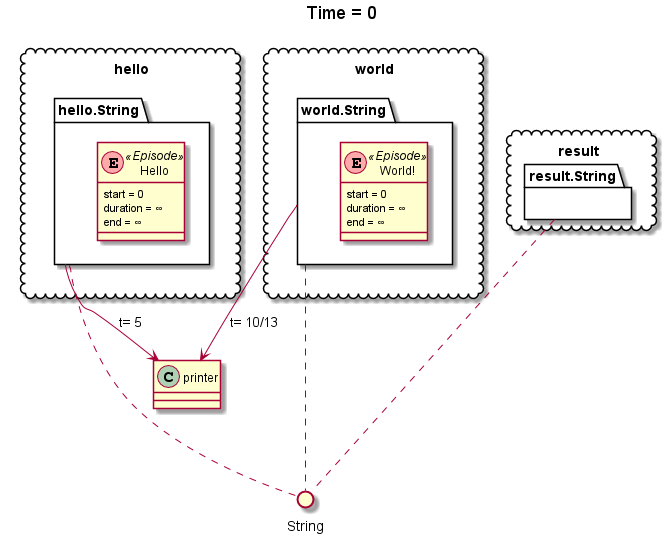
\includegraphics[width=0.7\linewidth]{state0}
	\caption{Визуализация примера из листинга \ref{list:interface}. Состояние 1.}
	\label{fig:state1}
\end{figure*}

\begin{figure*}[h]
	\centering
	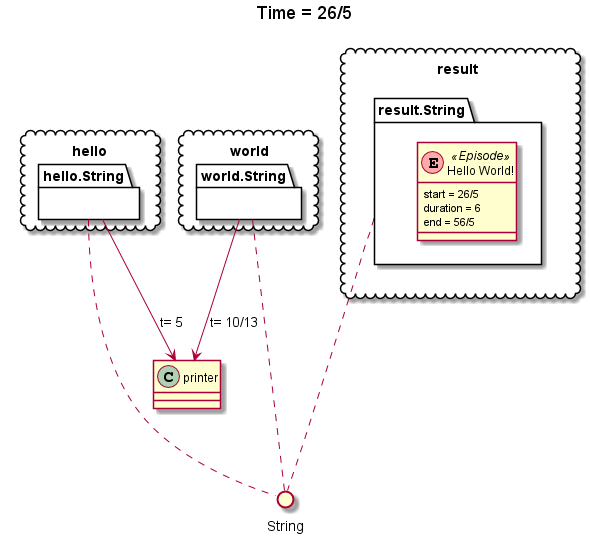
\includegraphics[width=0.7\linewidth]{state1}
	\caption{Визуализация примера из листинга \ref{list:interface}. Состояние 2.}
	\label{fig:state2}
\end{figure*}


%\section{Пример работы}
\begin{figure*}[h]
	\centering
	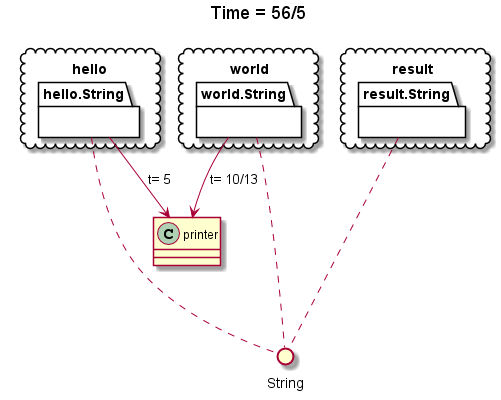
\includegraphics[width=0.7\linewidth]{state2}
	\caption{Визуализация примера из листинга \ref{list:interface}. Состояние 3.}
	\label{fig:state3}
\end{figure*}

\chapter{Пример нахождения НОД алгоритмом Евклида} \label{AppendixB}

\lstinputlisting[lastline=264, language={Kotlin}, caption={Реализация алгоритма Евклида на языке динамических систем.}, label={list:euclidean}] {listings/euclidean.kt}

\begin{figure*}[h]
	\centering
	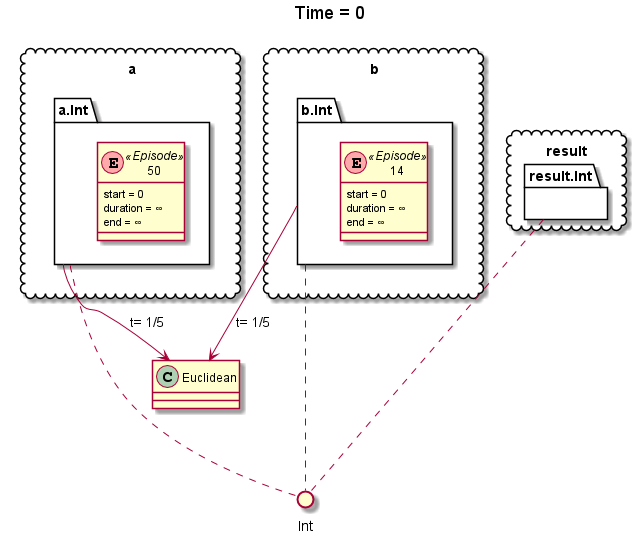
\includegraphics[width=0.7\linewidth]{images/euclidean1}
	\caption{НОД(50,14). Состояние 1.}
	\label{fig:euclidean1}
\end{figure*}
\begin{figure*}[h]
	\centering
	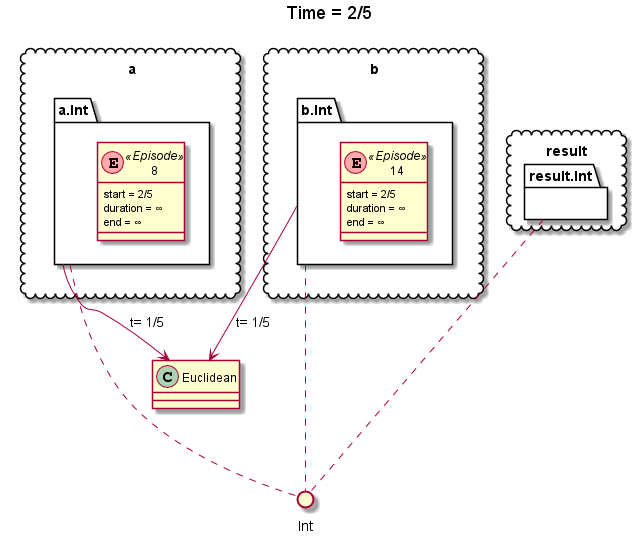
\includegraphics[width=0.7\linewidth]{images/euclidean2}
	\caption{НОД(50,14). Состояние 2.}
	\label{fig:euclidean2}
\end{figure*}
\begin{figure*}[h]
	\centering
	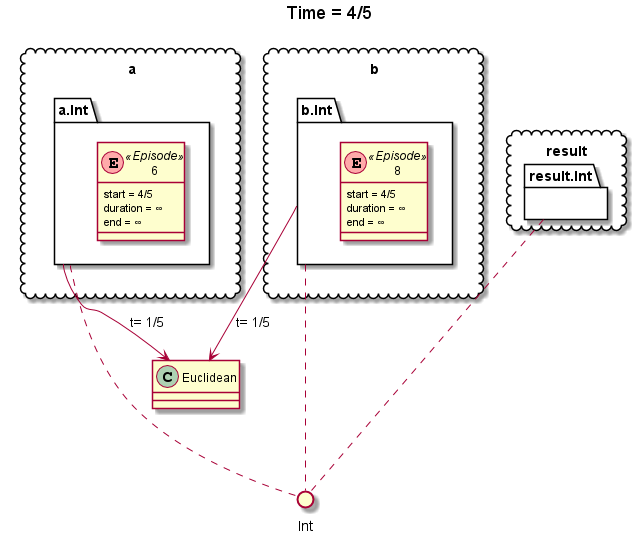
\includegraphics[width=0.7\linewidth]{images/euclidean3}
	\caption{НОД(50,14). Состояние 3.}
	\label{fig:euclidean3}
\end{figure*}
\begin{figure*}[h]
	\centering
	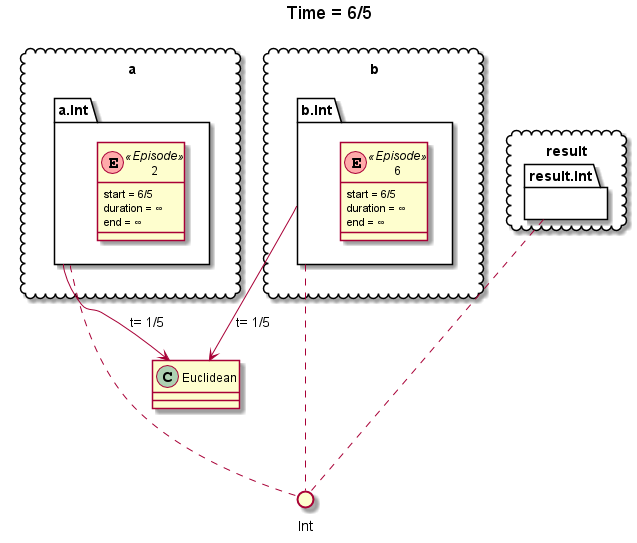
\includegraphics[width=0.7\linewidth]{images/euclidean4}
	\caption{НОД(50,14). Состояние 4.}
	\label{fig:euclidean4}
\end{figure*}
\begin{figure*}[h]
	\centering
	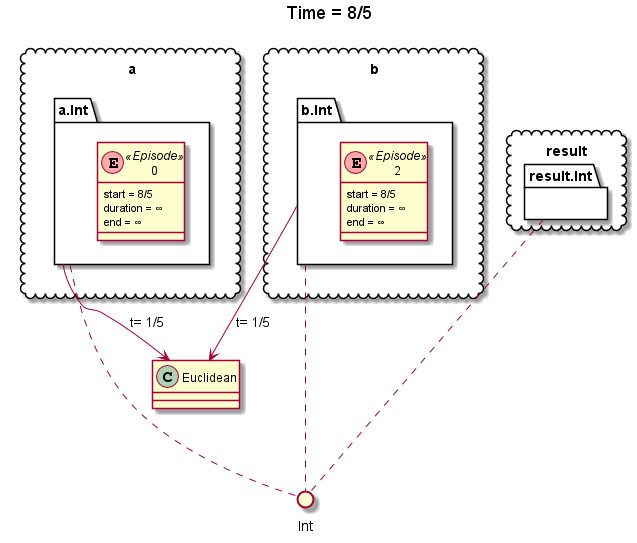
\includegraphics[width=0.7\linewidth]{images/euclidean5}
	\caption{НОД(50,14). Состояние 5.}
	\label{fig:euclidean5}
\end{figure*}
\begin{figure*}[h]
	\centering
	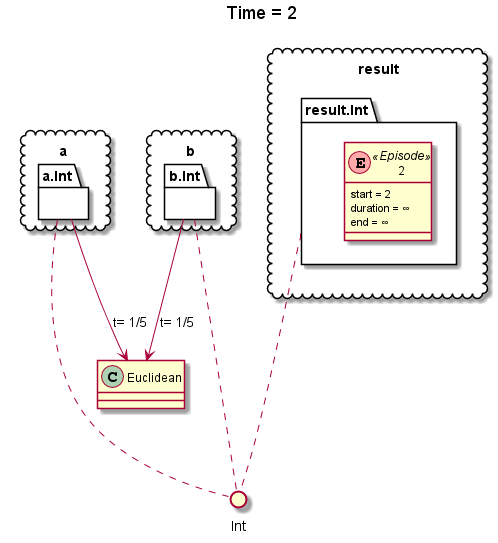
\includegraphics[width=0.5\linewidth]{images/euclidean6}
	\caption{НОД(50,14). Состояние 6. Результат.}
	\label{fig:euclidean6}
\end{figure*}



\chapter{Исходный код программы}
\lstinputlisting[lastline=264, language={Kotlin}, caption={DataModel.kt}, label={list:datamodel}] {listings/DataModel.kt}

\lstinputlisting[lastline=66, language={Kotlin}, caption={DSL}, label={list:dsl}] {listings/DSL.kt}


\lstinputlisting[lastline=96, language={Kotlin}, caption={Time.kt}, label={list:time}] {listings/Time.kt}

\lstinputlisting[lastline=129, language={Kotlin}, caption={Process.kt}, label={list:process}] {listings/Process.kt}

\lstinputlisting[lastline=62, language={Kotlin}, caption={PlantUML.kt}, label={list:plantuml}] {listings/PlantUML.kt}        % Приложения

\end{document}
